% UG project example file, February 2022 Do not change the first two lines of
% code, except you may delete "logo," if causing problems. Understand any
% problems and seek approval before assuming it's ok to remove ugcheck.
\documentclass[logo,bsc,singlespacing,parskip]{infthesis}
\usepackage{ugcheck}
\newcommand{\todo}{\textbf{?} }
\usepackage{color,soul}
% \usepackage{hyperref}
\usepackage{graphicx}
\usepackage{array}
\usepackage{xcolor}
\usepackage{soul}
\usepackage{booktabs}
\usepackage{fancyvrb}
\usepackage{relsize}
\usepackage{float}
\usepackage[hidelinks]{hyperref}
\usepackage{tikz}

\newcommand{\sigfpe}{\texttt{SIGFPE}}
\newcommand{\dthalfi}{\texttt{int10\char`_t}}
\newcommand{\dtshort}{\texttt{int16\char`_t}}
\newcommand{\dtint}{\texttt{int32\char`_t}}
\newcommand{\dtlong}{\texttt{int64\char`_t}}
\newcommand{\dthalf}{\texttt{half}}
\newcommand{\dtfloat}{\texttt{float}}
\newcommand{\dtfloati}{\texttt{int23\char`_t}}
\newcommand{\dtdouble}{\texttt{double}}
\newcommand{\dtdoublei}{\texttt{int52\char`_t}}
\newcommand{\feinexact}{\texttt{FE\char`_INEXACT}}
\newcommand{\feinvalid}{\texttt{FE\char`_INVALID}}
\newcommand{\mxcsr}{\texttt{mxcsr}}
\newcommand{\pivot}{\texttt{pivot}}
\newcommand{\mca}{\texttt{llvm-mca}}
\newcommand{\exegesis}{\texttt{llvm-exegesis}}
\newcommand{\xmm}{\texttt{XMM}}
\newcommand{\ymm}{\texttt{YMM}}
\newcommand{\zmm}{\texttt{ZMM}}

\newenvironment{VerbatimCompact}
  {\vspace*{-2.5mm}\VerbatimEnvironment
   \par\Verbatim}
  {\endVerbatim\vspace*{-2.4mm}}


\newcolumntype{V}[1]{>{\topsep=0pt\@minipagetrue}p{#1}<{\vspace{-\baselineskip}}}
\makeatother
\newcommand{\command}[1]{\texttt{\string#1}}

\newcommand{\hlc}[2][yellow]{{%
    \colorlet{foo}{#1}%
    \sethlcolor{foo}\hl{#2}}%
}

\newcolumntype{L}[1]{>{\raggedright\let\newline\\\arraybackslash\hspace{0pt}}m{#1}}
\newcolumntype{C}[1]{>{\centering\let\newline\\\arraybackslash\hspace{0pt}}m{#1}}
\newcolumntype{R}[1]{>{\raggedleft\let\newline\\\arraybackslash\hspace{0pt}}m{#1}}

\newenvironment{compactlist}
{ \begin{enumerate}
    \setlength{\itemsep}{0pt}
    \setlength{\parskip}{0pt}
    \setlength{\parsep}{0pt}     
}
{ \end{enumerate} } 

% Include any packages you need below, but don't include any that change the page
% layout or style of the dissertation. By including the ugcheck package above,
% you should catch most accidental changes of page layout though.

\usepackage{microtype} % recommended, but you can remove if it causes problems

\begin{document}
\begin{preliminary}

\title{Fast \pivot{} Function for MLIR's Presburger Library Through
Vectorization and Integer Arithmetic in FPU}

\author{Zhou Qi}

% CHOOSE YOUR DEGREE a):
% please leave just one of the following un-commented
% \course{Artificial Intelligence}
%\course{Artificial Intelligence and Computer Science}
%\course{Artificial Intelligence and Mathematics}
%\course{Artificial Intelligence and Software Engineering}
%\course{Cognitive Science}
\course{Computer Science}
%\course{Computer Science and Management Science}
%\course{Computer Science and Mathematics}
%\course{Computer Science and Physics}
%\course{Software Engineering}
%\course{Master of Informatics} % MInf students

% CHOOSE YOUR DEGREE b):
% please leave just one of the following un-commented
%\project{MInf Project (Part 1) Report}  % 4th year MInf students
%\project{MInf Project (Part 2) Report}  % 5th year MInf students
\project{4th Year Project Report}        % all other UG4 students


\date{\today}

\abstract{
\label{sec:abstract}

This report presents a fast implementation of the core function \pivot{} for a
math library in MLIR by performing vectorized integer arithmetics in
FPU. The hot loop of the \pivot{} function performs overflow-checked
multiplication and addition on each element of an input matrix of low dimension
and mostly small-value items. MLIR's upstream uses element-wise
transprecision computing, where the data type of each element starts with 
\dtlong{}, and will be switched to \texttt{LargeInteger} in case of overflow. 
Compilers cannot automatically vectorize this approach, and
\dtlong{} has a much larger bit width than what is
typically needed for most items in the matrix.
Additionally, extra arithmetics are required to perform overflow checking 
for integers, resulting in significant overhead.
These issues can be addressed by taking
advantage of SIMD, and reducing the bit width for every element. 
This report also introduces the \dtfloati{}
data type, a 23-bit integer data type created from the 23-bit mantissa of a
32-bit floating point.
\dtfloati{} overflow can be captured as floating point imprecision by a
status register, making overflow awareness almost free.  
On a selected 30-row by 19-column representative input matrix, the runtime is
reduced from 550 ns to 26 ns, achieving 20 times speedup.

% This can be improved if hardware resources are utilized effectively, by taking
% advantage of SIMD, and reducing the bit width for every element. 

}

\maketitle

\newenvironment{ethics}
   {\begin{frontenv}{Research Ethics Approval}{\LARGE}}
   {\end{frontenv}\newpage}

\begin{ethics}

This project was planned in accordance with the Informatics Research
Ethics policy. It did not involve any aspects that required approval
from the Informatics Research Ethics committee.

\standarddeclaration
\end{ethics}


\begin{acknowledgements}
    I would like to express my deepest gratitude to my supervisor, Tobias Grosser,
    for his invaluable guidance and support throughout this project. His
    innovative ideas and enthusiasm have inspired me, and working under his
    mentorship was a great opportunity. I have learnt a lot about computer
    architectures throughout this exciting project, this would not have been
    possible without his involvement.

    I am also grateful to Tobias's Ph.D. students, Arjun Pitchanathan
    and Sasha Lopoukhine. Arjun's assistance have been instrumental
    in the progress of this project. I want to extend special thanks to
    Sasha for generously granting me access to the powerful 7950x workstation.
    
    Finally, I would like to express my heartfelt appreciation to all my friends
    who have been a constant source of encouragement and motivation. A special
    mention goes to Emanon42, lyzh, gjz010, and Marisa Kirisame, their
    camaraderie and support have made this journey enjoyable and memorable.

\end{acknowledgements}


\tableofcontents
\end{preliminary}


\chapter{Introduction}
\label{sec:introduction}

MLIR, Multi-Level Intermediate Representation, is an infrastructure for building
reusable and extensible compilers. It aims to reduce fragmentation in domain-specific
languages and heterogeneous hardware~\cite{mlir}. Its Presburger
library provides polyhedral compilation techniques for dependence analysis,
loop optimization~\cite{mliraffine}, and cache modeling~\cite{CacheModel}.
Presburger arithmetics involves determining whether a linear problem is 
satisfiable under its constraints~\cite{SMLPPA}, and can be solved using the
simplex method of linear programming, with its core function \pivot{} is the
main performance bottleneck~\cite{FPL1}. 
% Presburger arithmetics involves determining whether the conjunction of linear
% arithmetic constraints is satisfiable~\cite{SMLPPA}, and can be solved using the
% simplex method of linear programming, with its core function \pivot{} is the
% main performance bottleneck~\cite{FPL1}. 


The \texttt{pivot} function involves two multiplication and one addition
operation on every element in a matrix. Notably, the input matrices for this
library tend to exhibit characteristics of small values and low dimensionality.
For example, 90\% of test cases work with 16-bit integers that never overflow,
and 74\% of the runtime is spent on test cases that we can compute using
16-bit integers and matrices with at most 32 columns~\cite{FPL2}. These
properties can be leveraged to utilize modern micro-architectural
hardware resources, thereby accelerating the process.

Currently, the source code in MLIR upstream adopts a nested for-loop to iterate
through every matrix element in a transprecision manner. Each element in
the matrix can either be \dtlong{} or \texttt{LargeInteger} and the
algorithm starts by using \dtlong{}. In case of overflow, it switches to
the \texttt{LargeInteger} version. This approach is computationally expensive
and inefficient, for the following reasons: 
\begin{enumerate}

\item \dtlong{} has a much larger bit width than what is typically
needed for most of the elements in the matrix.

\item The compiler is not capable of generating vectorized instructions from
scalar source code.

\item Overflow is checked through additional arithmetic
operations.

\end{enumerate}

To propose a faster alternative to the \texttt{pivot} function, we could
consider constructing a new \texttt{pivot} algorithm that satisfies the
following conditions:
\begin{enumerate}

\item Utilize SIMD: preliminary benchmark (Section
\ref{sec:vectorization-method-eval}) indicates at least 10 times
performance improvement. 

\item Use small bit width for every element: reducing the bit width by half
doubles the amount of elements packed into a single vector register, and
essentially reduces the instruction count by half (Table \ref{archtable}). 

\item Fast overflow checking: overflow has to be checked manually for integers,
which introduces at least 65\% overhead toward total runtime (Section
\ref{sec:i16-overflow-checking}). This is because the x86 architecture does not
provide status registers to indicate vectorized integer overflow. However, there
is one for floating points, making overflow detection for vector floating point
operations almost free. 

\end{enumerate}


Previously there was an attempt to vectorize \texttt{pivot} that utilizes
\dtshort{} and targets matrices with 32 columns or less~\cite{FPL2}. This
approach offers the advantage of being able to pack a row of 32 elements into a
single AVX-512 register and addresses issues 1 and 2. However, overflow
is still checked manually, causing 4 times more instruction count (Section
\ref{sec:i16-overflow-checking}). Additionally, this approach introduces a new
drawback. The AVX-512 extension is required for CPUs to support
vectorized \dtshort{}, and this is very rare among CPUs manufactured in the last
decade (Section \ref{sec:avx512}). 

An alternative approach is to do 24-bit or 53-bit integer operations using float
(32-bit floating point) or double (64-bit floating point)\footnote{ IEEE 754 specification is introduced in Section
\ref{sec:IEEE754}}. 
Though
floating points are notorious for precision issues, they are reliable when
representing integers that fit inside their mantissa. 
% The bit width of 
% precise integer is up to 24 bits for float and 53
% bits for double
Here, ``overflow'' can be defined as imprecision, rather than a restriction on 
bit width. 
When the result of some integer computation exceeds the bit
size of the mantissa, floating point imprecision almost always occurs and a
status register will be set automatically. Occasionally, imprecision does not
happen due to floating point normalization, and this is not considered as
overflow.
(Section \ref{sec:overflow-float}).

Comparing to \dtshort{}, since the overflow checking overhead can be
significantly reduced, using floating points could potentially be faster.
However it comes with the cost of larger bit width and smaller vector size, as
there does not exist support for 16-bit floating point \texttt{half}. The cost
of overflow checking for floating points is the time spent on resetting the
status register once at the beginning of a sequence of calls to
\pivot{}~\cite{FPL1}, plus reading it in each \pivot{} call. Even though reading
the register takes 5 ns and resetting it costs 10.5 ns (Figure \ref{plot_fenv}),
the effective total overhead can be less than 1 ns through optimization (Figure
\ref{fig:specialization}). The superscalar and out-of-order execution pipeline
hides the latency of reading the status register. Also, the \pivot{} function is
often invoked repeatedly in a sequence \cite{FPL1}, making the cost of resetting
the status register negligible for each single call. 



Another advantage of \dtfloat{} over \dtint{} is that floating points offer
better compatibility with old computers. Vectorized \dtfloat{} implementation of
\pivot{} runs fine with AVX-2, it does not require new features from the AVX-512
extension. Thus it is possible to be executed on almost every x86 CPU from the
last decade. 
% It can also be adapted to
% fit even older \texttt{AVX-128} and SSE CPUs with slight change in the
% source code.

This report will first analyze the capability of modern CPU micro-architecture,
especially Zen 4, through a matrix element-wise fused-multiply-add toy
example under the various configurations regarding vectorization methods, matrix
data structures, element data types, and data widths (Section \ref{sec:Toy}). 
It is discovered that optimal performance can be achieved by selecting Clang
vector type extension as the vectorization methods, and using a flat list as the
matrix data structure. However, it is quite difficult to decide whether
\dtshort{} or \dtfloat{} is better, because the former benefits from bigger
vector size and less instruction count, while the latter has a minimal overhead
on overflow checking. 

Then two detached versions of \texttt{pivot} function from the Presburger
library are built, according to the most optimal configurations from the toy
example, one using \dtshort{} and the other using \dtfloat{}. After applying 
further optimizations (Section \ref{sec:pivot-impl}), a benchmark is set up for a
selected 30-row and 19-column matrix. The achievements are: 
\begin{enumerate}
    \item The vectorized \dtfloat{} implementation of \pivot{} significantly
    outperforms the upstream. Specifically, it takes only 26 ns, while the
    runtime of the upstream implementation is 550 ns. 
    % ,  \dtshort{} completes 6 ns ahead.
    % , which renders the 6 ns gap trivial. 
    \item The \dtfloat{} implementation offers substantial compatibility
    advantage over \linebreak \dtshort{} for the vast amount of non-AVX-512
    platforms. Even though the \dtshort{} version is 6 ns faster than the
    \dtfloat{} version, the significant improvement from the upstream 
    together with AVX-2's compatibility
    renders the 6 ns gap trivial. 
\end{enumerate}

%The column of the matrix can be configured to be 8, 16, 24 or 32.
% In the case of 24 columns, which is considered to be the most representative
% case~\cite{FPL1}

\chapter{Background}
\section{Linear Programming and Simplex Algorithm}
\label{simplex}
Linear programming is a mathematical optimization technique used to model and
find the best possible solution to a problem, using a set of constraints and 
the objective function to maximize or minimize. Its canonical form consists of a
objective function:
\begin{math}
Z = c_1x_1 + c_2x_2 + ... + c_nx_n
\end{math}, subjecting to the constraints: \\
\begin{math}
x_1 \, ... \, x_n \ge 0
\end{math}\\
\begin{math}
a_{11}x_1 + a_{12}x_2 + ... + a_{1n}x_n = b_1 
\end{math}\\
\begin{math}
a_{21}x_1 + a_{22}x_2 + ... + a_{2n}x_n = b_2
\end{math}\\
\begin{math}
...
\end{math}\\
\begin{math}
a_{m1}x_1 + a_{m2}x_2 + ... + a_{mn}x_n = b_m
\end{math}, \\
where \begin{math}x_1 \,...\, x_n\end{math} are the variables, 
\begin{math}c_1 \,...\, c_n\end{math} are the coefficients of the objective function, 
and non-negative \begin{math}a_{11}, a_{12} \,...\, a_{21} \,...\ a_{m1} \,...\, a_{mn}\end{math}
together with \begin{math}b_1 \,...\, b_m\end{math} encodes the constraints of
the problem in a matrix \cite{FPL1}. 

% For example, the constraints 
% \begin{math}
% x_1 + x_2 \geq 10
% \end{math}
% and 
% \begin{math}
% 7x_1 - 4x_2 \leq 5
% \end{math} can be normalized into 
% \begin{math}
% x_1 + x_2 - 10 \geq 0
% \end{math}
% and 
% \begin{math}
% -7x_1 + 4x_2 + 5 \geq 0
% \end{math}
    
The simplex algorithm is an iterative approach to find \begin{math} x_1 \, ...
\, x_n\end{math} that maximizes the objective function while satisfying
constraints at the same time. The matrix goes through a sequence of
transformations, until the solution appears or it is found that the solution is
not feasible. The transformations are called ``pivot'', and it solves the linear
equation at the pivot row for the variable at the pivot column: 
\vspace*{-4mm}
\begin{table}[H]
\begin{center}
\begin{tabular}{llll}
Pivot item           & $\alpha$ & $\rightarrow$ & $\frac{1}{\alpha}$            \\
Rest of the pivot row    & $\beta$  & $\rightarrow$ & $-\frac{\beta}{\alpha}$            \\
Rest of the pivot column& $\gamma$ & $\rightarrow$ & $\frac{\gamma}{\alpha}$            \\
Other entries         & $\delta$ & $\rightarrow$ & $\delta - \frac{\beta\gamma}{\alpha}$  
\end{tabular}
\end{center}
\end{table}
\vspace*{-8mm}

The pivot transformation involves division and thereby produces rational
numbers. Rationals of base 10 cannot be expressed as binary floating points
precisely due to inaccuracy caused by potential rounding. In addition, divisions
are expensive operations compared to additions or multiplications. This issue
can be addressed through the denormalization of rows, by multiplying each row with
their common denominator~\cite{FPL1}: 
\vspace*{-4mm}
\begin{table}[H]
\begin{center}
\begin{tabular}{llll}
Pivot item           & $\alpha$ & = & $\frac{\alpha_n}{d_p}$            \\
Rest of the pivot row    & $\beta$  & = & $\frac{\beta_n}{d_p}$            \\
Rest of the pivot column& $\gamma$ & = & $\frac{\gamma_n}{d_i}$            \\
Other entries         & $\delta$ & = & $\frac{\delta_n}{d_i}$  
\end{tabular}
\end{center}
\end{table}
\vspace*{-8mm}
where $d_p$ is the denominator of the pivot row, $d_i$ is the denominator of the
$i^{th}$ row. After demoralization $\alpha_n$, $\beta_n$, $\gamma_n$, and
$\delta_n$, becomes $\alpha$, $\beta$, $\gamma$, and $\delta$.

Substituting into the processing formula, the pivot row becomes:
\vspace*{-4mm}
\begin{table}[H]
\begin{center}
\begin{tabular}{llll}
Pivot item           & $\frac{\alpha_n}{d_p}$ & $\rightarrow$ & $\frac{d_p}{\alpha_n}$       \\
Rest of the pivot row    & $\frac{\beta_n}{d_p}$  & $\rightarrow$ & -$\frac{\beta_n}{\alpha_n}$  
\end{tabular}
\end{center}
\end{table}
\vspace*{-8mm}
This transformation effectively becomes swapping $\alpha_n$ with $d_p$ and
negating every non-pivot-column item. 

Likewise, the non-pivot rows are transformed as the following:
\vspace*{-4mm}
\begin{table}[H]
\begin{center}
\begin{tabular}{llll}
Rest of the pivot column& $\frac{\gamma_n}{d_i}$ & $\rightarrow$ & $\frac{\gamma_nd_p}{a_nd_i}$            \\
Other entries         & $\frac{\delta_n}{d_i}$    & $\rightarrow$ & $\frac{\delta_na_n-\beta_n\gamma_n}{a_nd_i}$  
\end{tabular}
\end{center}
\end{table}
\vspace*{-8mm}
and can be implemented in these procedures: 
\vspace*{-2.0mm}
\begin{compactlist}
    \item Update row denominator: $d_i' = d_ia_n$, 
    \item Multiply non-pivot-column items by $a_n$,
    \item Subtract $\beta_n\gamma_n$ from every non-pivot row.
\end{compactlist}

\section{Presburger Library}
\label{sec:presburger}
% \subsection{Overview}

The Fast Presburger Library (FPL) paper collected 465,460 representative linear
programming problems encountered during cache analytical
modeling, polyhedral loop optimization, and accelerator code generation. It is
found that most of the constraint matrices are low in dimensionality and small
in the value of each element~\cite{FPL1}. Specifically, more than 99\% of the
entries from matrices require less than 10 bits, and 95\% of them are less than 20 columns
(Figure \ref{small-val-low-dim}). Thus, most rows fit inside a 512-bit
vector register of 32 \dtshort{} elements, and a row operation can be done in a
single instruction. 


\begin{figure}
    \begin{center}
        %\captionsetup{justification=centering}
    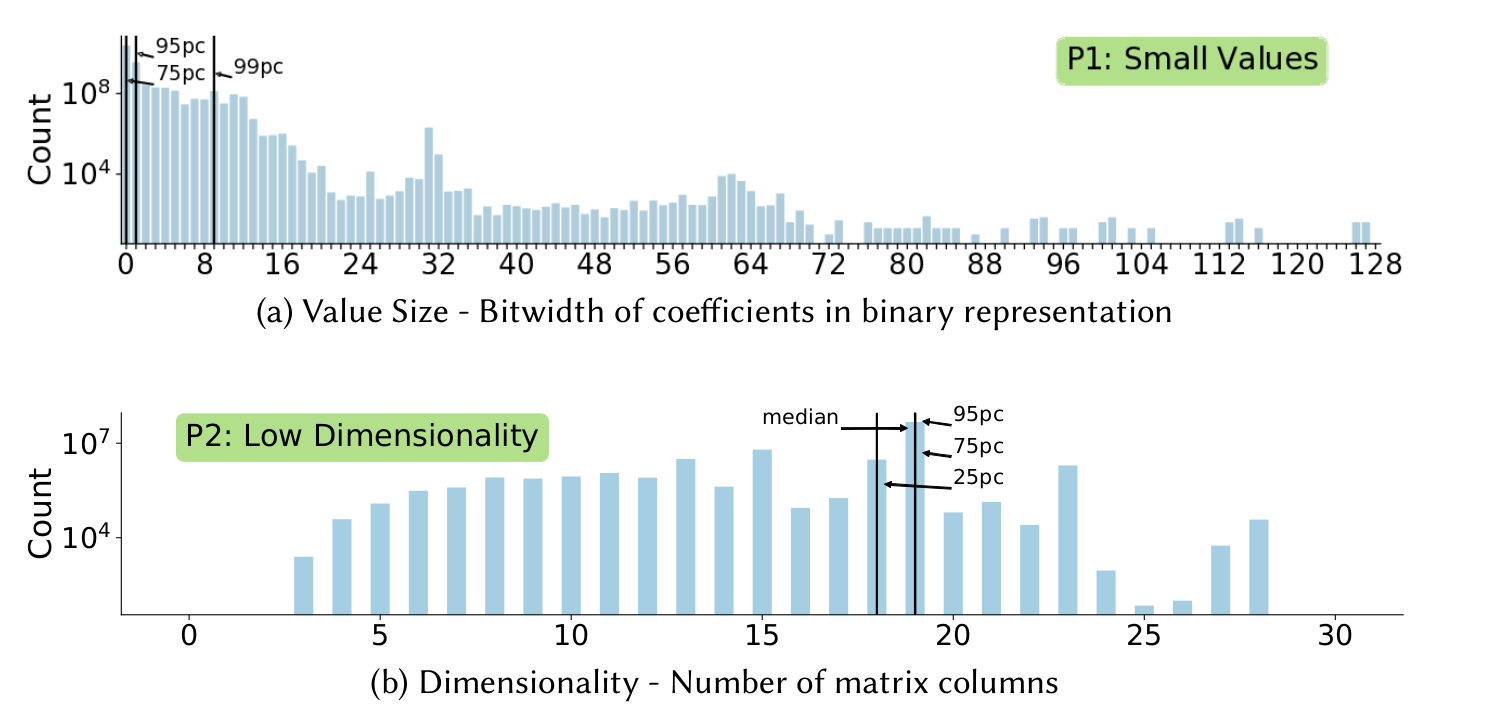
\includegraphics[width=\linewidth]{image/small-val-low-dim.png}
    \caption{Linear programming problems for program analysis exhibits unique
    characteristics of small value size and low dimensionality~\cite{FPL1}.}
    \label{small-val-low-dim}
    \end{center}
\end{figure}


However, in rare and corner cases, large coefficients can be up to 127 bits.
Practically, the upper bound of coefficient size is unknown, making it required
to have arbitrary precision arithmetic \texttt{LargeInteger} as a backup. Also,
the maximum observed column count is 28, and there is no specific maximum column
count. 

The FPL paper presents a 3-way transprecision implementation for the Presburger
library's simplex solver using the algorithm described in Section \ref{simplex}.
It starts from row-wise vectorized \dtshort{}, and will switch to  element-wise
scalar \dtlong{} or element-wise scalar \texttt{LargeInteger} in case of
overflow, as illustrated in Figure \ref{fig:fpl_arch}. Unfortunately the
MLIR upstream only presents a 2-layer transprecision, consisting of element-wise
scalar operation using \dtlong{} and \texttt{LargeInteger}. The \dtshort{}
version is not merged with the upstream for two reasons: 
\begin{compactlist} 
    \item \dtshort{} vectors require AVX-512 ISA extension, but hardware
    support is rare (Section \ref{sec:avx512}). 
    \item Despite the \dtshort{} version being fast, overflow checking overhead
    is 65\%~\cite{FPL2}. Using floating points could significantly reduce this
    overhead and potentially be faster (Section \ref{sec:i23}).  
\end{compactlist}


\begin{figure}
    \begin{center}
        %\captionsetup{justification=centering}
    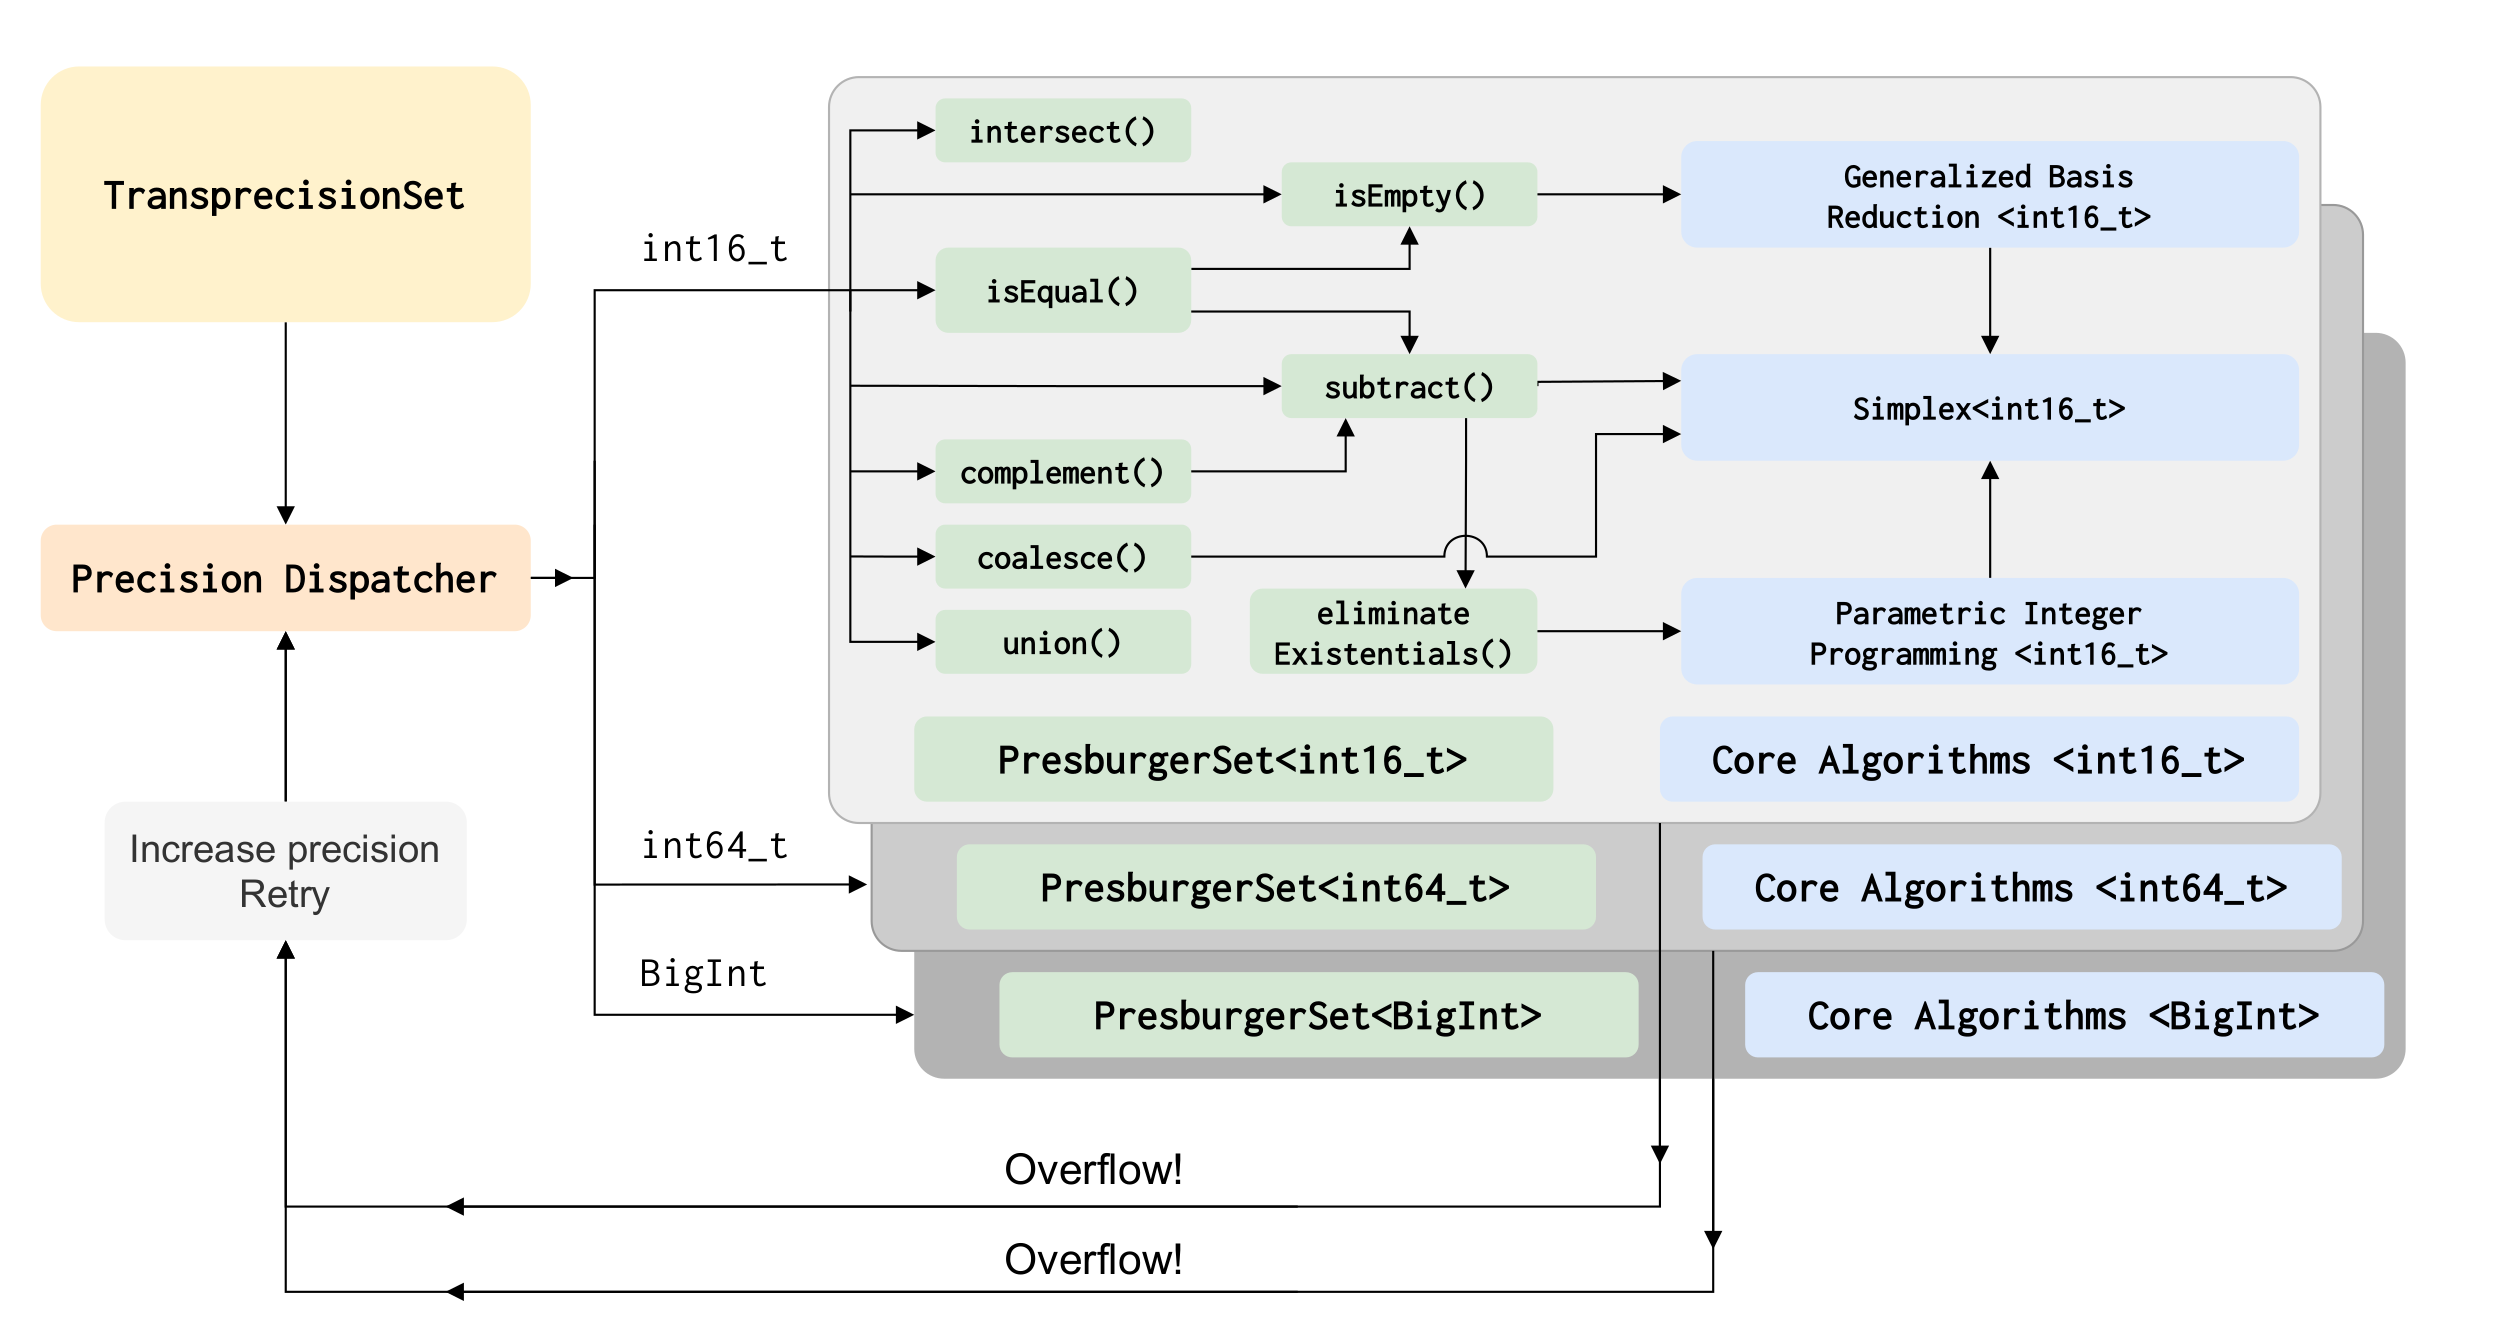
\includegraphics[width=\linewidth]{image/transprecision.png}
    \caption{The architecture of FPL. The focus of this report is the
    ``Simplex'' method of the ``Core Algorithms'', since it is the main
    performance bottleneck.~\cite{FPL2}}
    \label{fig:fpl_arch}
    \end{center}
\end{figure}

\section{Modern CPU Micro-architecture}
\label{sec:avx512}

A recent trend in the development of the x86-64 architecture is to include AVX-512
instruction set architecture (ISA) extension. AVX-512 succeeds AVX-2, the vector
width is increased from AVX-2’s 256 bits to 512 bits. AVX-512 also provides new
instructions, for example, \dtshort{} saturated addition.

% \subsection{Intel}

Even though its specification was released by Intel in 2013, it had been
unpopular ~\cite{linusHopeAvx512Die}, as it did not bring practical performance
improvements. The primary reason was that it consumed much more power than
usual, causing severe overheating. A classic example is the micro-architecture
Skylake from Intel and its AVX-512 enabled counterpart Skylake-X.
Skylake has 2 256 bits FMA AVX-2 execution
units\footnote{Fused-multiply-add (FMA) execution units are a type of floating
point execution units, capable of doing addition, multiplication, or both in a
single instruction. See Section \ref{sec:FMA}.}. For Skylake-X Intel provides 2
512-bit AVX-512 FMA units by fusing the existing AVX-2 units
into a AVX-512 unit, then introduces an additional FMA AVX-512
unit~\cite{SLK-X}. The additional AVX-512 unit increases the heat flux
density of the chip, causing server thermal throttling issues. 

Intel attempted to mitigate this problem by introducing the
``AVX-offset'' mode. When a workload involving AVX-512
instructions is encountered, the CPU automatically enters the
AVX-offset mode and reduces its clock frequency \cite{AVX-offset}. This
solution only works in theoretical benchmarks where AVX-512
instructions are present in large bulk, but in practice, it is more common to have a
mix of control flow, scalar, SSE and AVX-512 instructions. The
clock frequency of executing those non-AVX-512 instructions is
decreased together with AVX-512 instructions, causing many workloads
could run faster with disabled AVX-512 and higher clock
frequency~\cite{Zen4Critique}. 

% \hlc[pink]{OptionalTODO: alderlake disabled avx-512 for big.LITTLE}


% \subsection{AMD}
AMD recently decided to add support for AVX-512 in their latest
micro-architecture Zen 4. It has slightly less computing power than
Intel but is much more efficient. Zen 4 can be considered as the modernized version of
Zen 3 or Zen 2, where Zen 2 and Zen 3 support AVX-2  by providing 2 FADD
units\footnote{Floating-point add units (FADD) can execute floating point addition
 instructions only. They are less capable compared to FMA.} and 2 FMA units of
256-bit width \cite{Zen2ChipWiki}. Zen 4 ``double-pumps'' these existing circuits
to create a single 512-bit FADD and a single 512-bit FMA, without introducing
any new arithmetic units ~\cite{Zen4Critique}. Zen 2 and Zen 3 are reputable for
their high performance per watt~\cite{ZenPerfPerWatt}, and Zen 4 would be better
with its more advanced lithography~\cite{Zen4Critique}.

Additionally, rebuilding existing software to target AVX-512 may
improve performance. One benefit of AVX-512 is that it reduces
front-end pressure. In the Zen 4 micro-architecture case, though the back-end is
possible to commit 2 AVX-2 FADD and 2 AVX-2 FMA every cycle,
the front-end has to dispatch 4 instructions per cycle, which is quite
difficult. The equivalency in AVX-512 only takes 2 instructions, and
this is much more likely to be sustained by the frontend~\cite{Zen4Critique}.


\section{Floating Points}
\label{sec:i23}
\subsection{IEEE 754}
\label{sec:IEEE754}
IEEE 754 is the standard for representing and manipulating floating-point
numbers in modern x86 computers. The standard defines several formats
for representing floating point numbers. The most common ones are 32-bit single
precision (\dtfloat{}) and 64-bit double precision (\dtdouble{}). For each format, the 
specification
defines how many bits are used to represent the sign, the exponent, and the mantissa. 

As Figure \ref{fig:ieee-f32} shows, the sign bit is a single bit that indicates whether the
floating point number is positive or negative. There are 8
bits and 11 bits for exponent in float and double, respectively, representing
the order of magnitude. The remaining 23 bits in float and 52 bits in double are
mantissae, the fractional part of the number is stored here. The value of a floating
point number can be computed through this formula: 
\begin{math} (-1)^s * 2^{(e - B)} * (1 + f)\end{math}
where \begin{math}s\end{math} is sign, \begin{math}e\end{math} is exponent, 
\begin{math}f\end{math} is mantissa and \begin{math}B\end{math} is a constant bias
value: \begin{math}127\end{math} for float, \begin{math}1023\end{math} for double. 

Figure \ref{fig:ieee-f32} provides an example of \dtfloat{} by presenting
\texttt{0.15625} in binary form:
\begin{VerbatimCompact}
sign     = 0b0        -> 0
exponent = 0b01111100 -> 0b01111100 - 127 = 124 - 127 = -3
mantissa = 0b01       -> 0b1.01 = 1.25
\end{VerbatimCompact}
Substituting the sign, the exponent, and the mantissa into the formula, we get: \\
\texttt{-1\^{}0 * 2\^{}(-3) * 1.25 = 0.15625}.



\begin{figure}
    \begin{center}
        %\captionsetup{justification=centering}
        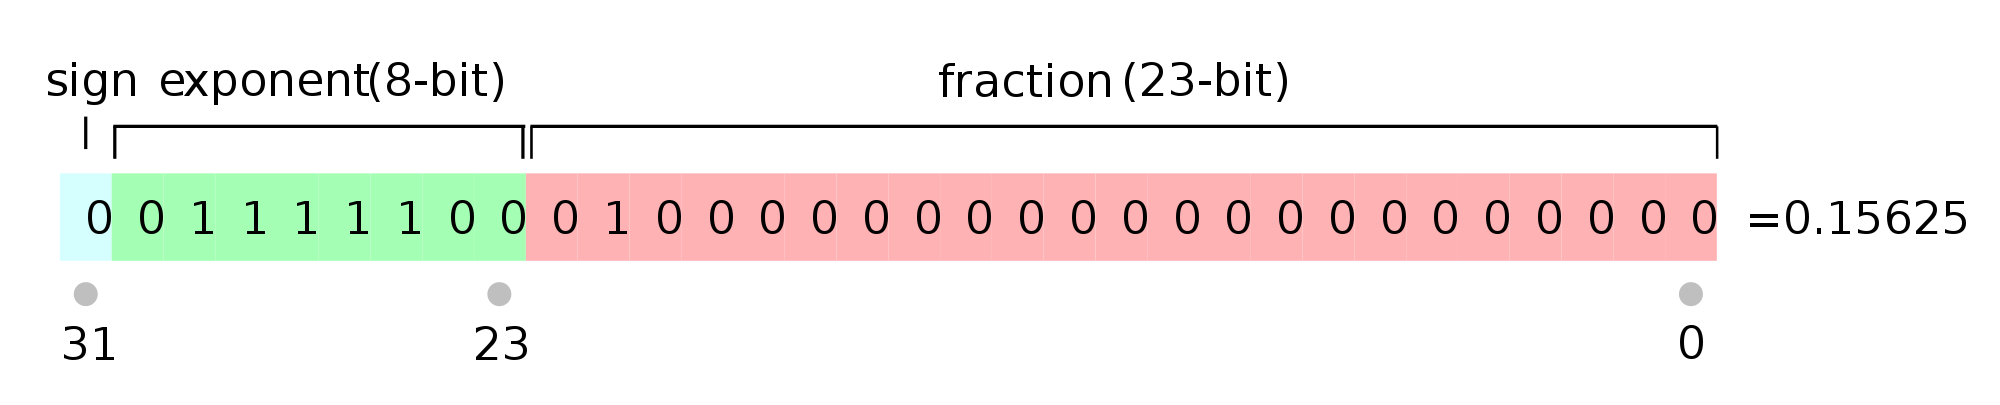
\includegraphics[width=\linewidth]{image/ieee-f32.png}
        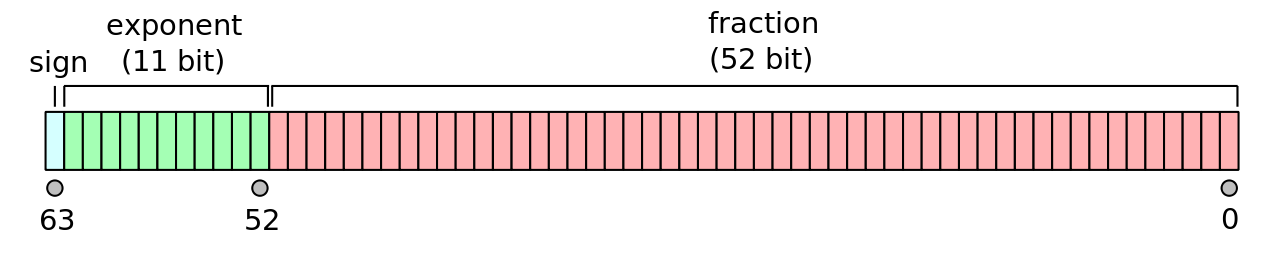
\includegraphics[width=\linewidth]{image/ieee-f64.png}
        \caption{IEEE 754 specification for single (32 bits) and double (64
        bits) precision floating point~\cite{ieee754-diagram}. In some
        literature ``mantissa'' is referred as ``fraction''.}
        \label{fig:ieee-f32}
    \end{center}
\end{figure}

\subsection{Fused-multiply-add}
\label{sec:FMA}

After doing floating point arithmetic, it is required to normalize the result of
floating-point arithmetic before it can be used further. However, by feeding the
result of a floating-point multiplication (FMUL) directly into the
floating-point addition (FADD) logic without the need for normalization and
rounding in between, a fused-multiply-add (FMA) operation is effectively
created: 
\begin{math}Y = (A * B) + C \end{math}, where 
\begin{math}A\end{math},
\begin{math}B\end{math} and
\begin{math}C\end{math} are the operands, 
\begin{math}Y\end{math} is the result~\cite{CARD}.

FMA saves cycles and reduces the accumulation of rounding errors, while at the same
time not adding significant complexity to the circuit. An FMA execution unit is
capable of doing FMUL, FADD, and FSUB as well: 
\begin{compactlist} 
\item[] Addition: \begin{math}Y = (A * 1.0) + C \end{math} 
\item[] Multiplication: \begin{math} Y = (A * B) + 0.0 \end{math} 
\item[] Subtraction: \begin{math} Y = (A * -1.0) + C\end{math} 
\end{compactlist} 

This feature is useful in many numerical computations involving
simultaneous multiplication and addition operations, such as dot products and
matrix multiplications. Since the \pivot{} function performs multiplications and
additions between the pivot row, some constant value, and each row in the matrix,
the performance of FMA is critical to the overall efficiency of the algorithm. 

\subsection{Representing ``\dtfloati{}'' and ``\dtdoublei{}'' \\ Using Floating Points}
\label{sec:fpe2}

There is a common stereotype that floating-point numbers are unreliable and
likely to be imprecise, and are often illustrated in popular memes as shown in
Figure \ref{meme}~\cite{meme}. However, when storing integer values inside
floating points, floating points can be pretty reliable. Historically
floating point processing units in GPUs have been utilized for fast integer
arithmetic, for example, modular exponentiation and RSA
algorithms~\cite{intfpu-modexp}, because often the architecture of GPU prioritizes
the performance of floating points rather than integers. 

Given that the mantissa part of a float consists of 23 bits,
inexactness never occurs when representing integers less than 23 bits (ignoring
the sign bit). Furthermore, in case of an integer overflow, floating point
imprecision almost always occurs, and setting a corresponding status register.
The same concept applies to double data types, which have a mantissa consisting
of 52 bits.

This mechanism is reliable, as floating-point inexactness always implies 
integer\linebreak-inexactness. For an integer value with a bit width bigger than the
mantissa size, floating point rounding is triggered to fit the most
significant bits of the integer in the mantissa, then adjust the order of
magnitude in the exponent accordingly. The lower bits of the mantissa are
truncated, therefore causing imprecision. 

In some rare cases, integers longer than the size of mantissa can be represented
in floating points precisely. An example of such numbers is a very large power
of 2, like \texttt{2\^{}30 = 0x40000000}. Its binary representation in
\dtfloat{} is:
\begin{VerbatimCompact}
Sign     = 0b0        -> 0     
Exponent = 0b10011011 -> 0b10011011 - 127 = 155 - 127 = 28             
Mantissa = 0b0        -> 0b1.0 = 1
\end{VerbatimCompact}
% -1^0 * 2^28 * 1 = 2^28 
Despite being greater than the size of
the mantissa, they are normalized rather than being rounded and therefore does
not break the mechanism of representing integers in floating points.


% \hl{TODO: place this paragraph here?}


\begin{figure}[H]
\begin{center}
    
\includegraphics[width=50mm,scale=0.1]{image/0.3004.jpg}
    \caption{A floating point meme: \texttt{0.1 + 0.2 =
    0.30000000000000004}~\cite{meme}.}
    \label{meme}
\end{center}
\end{figure}

\section{Google Benchmark}
Google benchmark is a library to measure the performance of a code snippet. It
provides unit-test-like interfaces to set up benchmarks around a code snippet
\cite{googlebench}. The given example from https://github.com/google/benchmark
is self-explanatory for its usage: 

\begin{verbatim}
#include <benchmark/benchmark.h>

static void BM_SomeFunction(benchmark::State& state) {
    // Perform setup here
    for (auto _ : state) {
    // This code gets timed
    SomeFunction();
    }
}
// Register the function as a benchmark
BENCHMARK(BM_SomeFunction);
// Run the benchmark
BENCHMARK_MAIN();
\end{verbatim}

The library first starts a timer, repeatedly executes its core loop: \linebreak
\texttt{for (auto \char`_ : state) ... } 
multiple times then pauses the timer. This method
ensures that the results are consistent and minimizes the overhead required for
recording the timing information. 

Executing the benchmarks will not only report both elapsed real-time and CPU
time, but also much other useful information to help reduce variance. 
\begin{verbatim}
Running ./build/example
***WARNING*** CPU scaling is enabled, the benchmark real-time 
measurements may be noisy and will incur extra overhead.
Run on (32 X 5800.00 MHz CPU s)
CPU Caches:
    L1 Data 32 KiB (x16)
    L1 Instruction 32 KiB (x16)
    L2 Unified 1024 KiB (x16)
    L3 Unified 32768 KiB (x2)
Load Average: 8.10, 5.14, 1.14
----------------------------------------------------------
Benchmark                Time             CPU   Iterations
----------------------------------------------------------
BM_SomeFunction       18.5 ns         18.5 ns     37935734
\end{verbatim}

The warning: ``CPU scaling is enabled, the benchmark real-time measurements may
be noisy and will incur extra overhead.'' is saying that the CPU clock frequency
is not consistent. The clock frequency is dynamically determined by the governor
algorithm according to the operating system. For example, with the
\texttt{performance} governor, the OS locks the CPU to the highest possible
clock frequency, specified at
\texttt{/sys/devices/system/cpu/cpu*/cpufreq/scaling\char`_max\char`_freq}. In
contrast, the \texttt{ondemand} governor will push the CPU to the highest
frequency on demand and then gradually reduce the frequency as the idle time
increases \cite{archLinuxFreqScal}.

However, the clock frequency is also dependent on the manufacture and other hardware constraints.
By default, both Intel (Turbo Boost) and AMD (Precision Boost Overdrive) have
support for raising clock frequency, beyond the control of the governor
\cite{GoogleBenchReduceVariance}. On the other hand, CPUs have self-protecting
thermal throttling mechanisms that reduce their clock frequency and voltage when
it is too hot. 

The benchmark mentioned in this report were performed on an AMD 7950x desktop
computer. The computer system went through the following these setups for
consistent results:
\begin{compactlist}
    \item Set the governor to \texttt{performance}, 
    \item Disable AMD Precision Boost Overdrive (or Intel Turbo Boost), 
    \item Lock clock frequency at a 4.5 GHz, or any desired and feasible value,
    \item Make sure heat dissipation is working properly.
\end{compactlist}



\section{\mca{}}

\mca{}, LLVM Machine Code Analyzer, is a tool to analyze the performance of
executing some instructions on a specific CPU micro-architecture, according to
scheduling information provided by LLVM~\cite{llvm-mca}. 

By supplying \mca{} with a piece of assembly code and the target
micro-architecture codename, \mca{} reports various metrics to indicate how fast
the given instructions will execute on the specified micro-architecture. It
first summarizes the instruction per clock (IPC) and throughput of the entire
instruction block, then gives detailed information about each instruction,
including the number of uOps, latency, throughput, potential load, store, and side
effects. \mca{} also reports resource pressure regarding arithmetic units and
memory load or store units. When the optional \texttt{-timeline} flag is
prompted, \mca{} illustrates a timeline view of the analyzed code, showing how
instructions progress through the pipeline stages of the target processor. The
timeline helps understand the capability of complicated out-of-order superscalar
architecture. 

An example is provided below. The analysis from \mca{} indicates that a
\texttt{znver2} (Zen 2) CPU can repeatedly execute a combination of
\texttt{vmovaps}\footnote{\texttt{vmovaps} can be either vector float load or
store instruction, depending on how operands are structured~\cite{instruction}.}
and \texttt{vfmadd213ps}\footnote{\texttt{vfmadd213ps} is the instruction for
fused-multiply-add~\cite{instruction}.} instructions every 1.3 cycles, or 
equivalently 2.74 instructions per cycle. The output from \mca{} is slightly
modified and truncated to fit inside the page.
% $ cat x.s
% vmovaps (%rdx,%rsi,4),%ymm0
% vmovaps (%rcx,%rax,4),%ymm1
% vfmadd213ps (%r8,%rdi,4),%ymm0,%ymm1
% vmovaps %ymm1,(%r9,%rax,4)

\begin{verbatim}
$ llvm-mca-15 -timeline -mcpu=znver2 ./x.s 
Iterations:        100
Instructions:      400
Total Cycles:      146
Total uOps:        400

Dispatch Width:    4
uOps Per Cycle:    2.74
IPC:               2.74
Block RThroughput: 1.3

Instruction Info:
[1]: #uOps
[2]: Latency
[3]: RThroughput
[4]: MayLoad
[5]: MayStore
[6]: HasSideEffects (U)

[1] [2] [3]  [4] [5] [6] Instructions:
 1   8  0.33  *          vmovaps  (%rdx,%rsi,4), %ymm0
 1   8  0.33  *          vmovaps  (%rcx,%rax,4), %ymm1
 1   12 0.50  *          vfmadd213ps  (%r8,%rdi,4), %ymm0, %ymm1
 1   1  0.33      *      vmovaps  %ymm1, (%r9,%rax,4)

Resources:
[0]   - Zn2AGU0
[1]   - Zn2AGU1
[2]   - Zn2AGU2
...
[8]   - Zn2FPU0
[9]   - Zn2FPU1
[10]  - Zn2FPU2
[11]  - Zn2FPU3
[12]  - Zn2Multiplier

Resource pressure per iteration:
[0]  [1]  [2]  [3] [4] [5] [6] [7] [8]  [9] [10] [11] [12]   
1.33 1.33 1.34  -   -   -   -   -  0.50  -   -   0.50  -     

Resource pressure by instruction:
[0]  [1]  [2]  ... [11] Instructions:
0.01 0.38 0.61 ...  -   vmovaps  (%rdx,%rsi,4), %ymm0
0.23 0.68 0.09 ...  -   vmovaps  (%rcx,%rax,4), %ymm1
0.27 0.24 0.49 ... 0.50 vfmadd213ps  (%r8,%rdi,4), %ymm0, %ymm1
0.82 0.03 0.15 ...  -   vmovaps  %ymm1, (%r9,%rax,4)

Timeline view:
                0123456789      
Index 0123456789           

[0,0] DeeeeeeeeER    .    vmovaps  (%rdx,%rsi,4), %ymm0
[0,1] DeeeeeeeeER    .    vmovaps  (%rcx,%rax,4), %ymm1
[0,2] D=eeeeeeeeeeeeER    vfmadd213ps  (%r8,%rdi,4), %ymm0, %ymm1
[0,3] D=============eER   vmovaps  %ymm1, (%r9,%rax,4)
[1,0] .DeeeeeeeeE-----R   vmovaps  (%rdx,%rsi,4), %ymm0
[1,1] .DeeeeeeeeE-----R   vmovaps  (%rcx,%rax,4), %ymm1
[1,2] .D=eeeeeeeeeeeeER   vfmadd213ps  (%r8,%rdi,4), %ymm0, %ymm1
[1,3] .D=============eER  vmovaps  %ymm1, (%r9,%rax,4)
[2,0] . DeeeeeeeeE-----R  vmovaps  (%rdx,%rsi,4), %ymm0
[2,1] . DeeeeeeeeE-----R  vmovaps  (%rcx,%rax,4), %ymm1
...

\end{verbatim}


% [2,2] . D=eeeeeeeeeeeeER  .    . vfmadd213ps  (%r8,%rdi,4), %ymm0, %ymm1
% [2,3] . D=============eER .    . vmovaps  %ymm1, (%r9,%rax,4)
% [3,0] .  DeeeeeeeeE-----R .    . vmovaps  (%rdx,%rsi,4), %ymm0
% [3,1] .  DeeeeeeeeE-----R .    . vmovaps  (%rcx,%rax,4), %ymm1
% [3,2] .  D=eeeeeeeeeeeeER .    . vfmadd213ps  (%r8,%rdi,4), %ymm0, %ymm1
% [3,3] .  D=============eER.    . vmovaps  %ymm1, (%r9,%rax,4)
% [4,0] .   DeeeeeeeeE-----R.    . vmovaps  (%rdx,%rsi,4), %ymm0
% [4,1] .   DeeeeeeeeE-----R.    . vmovaps  (%rcx,%rax,4), %ymm1
% [4,2] .   D=eeeeeeeeeeeeER.    . vfmadd213ps  (%r8,%rdi,4), %ymm0, %ymm1
% [4,3] .   D=============eER    . vmovaps  %ymm1, (%r9,%rax,4)
% [5,0] .    DeeeeeeeeE-----R    . vmovaps  (%rdx,%rsi,4), %ymm0
% [5,1] .    DeeeeeeeeE-----R    . vmovaps  (%rcx,%rax,4), %ymm1
% [5,2] .    D=eeeeeeeeeeeeER    . vfmadd213ps  (%r8,%rdi,4), %ymm0, %ymm1
% [5,3] .    D=============eER   . vmovaps  %ymm1, (%r9,%rax,4)
% [6,0] .    .DeeeeeeeeE-----R   . vmovaps  (%rdx,%rsi,4), %ymm0
% [6,1] .    .DeeeeeeeeE-----R   . vmovaps  (%rcx,%rax,4), %ymm1
% [6,2] .    .D=eeeeeeeeeeeeER   . vfmadd213ps  (%r8,%rdi,4), %ymm0, %ymm1
% [6,3] .    .D=============eER  . vmovaps  %ymm1, (%r9,%rax,4)
% [7,0] .    . DeeeeeeeeE-----R  . vmovaps  (%rdx,%rsi,4), %ymm0
% [7,1] .    . DeeeeeeeeE-----R  . vmovaps  (%rcx,%rax,4), %ymm1
% [7,2] .    . D=eeeeeeeeeeeeER  . vfmadd213ps  (%r8,%rdi,4), %ymm0, %ymm1
% [7,3] .    . D=============eER . vmovaps  %ymm1, (%r9,%rax,4)
% [8,0] .    .  DeeeeeeeeE-----R . vmovaps  (%rdx,%rsi,4), %ymm0
% [8,1] .    .  DeeeeeeeeE-----R . vmovaps  (%rcx,%rax,4), %ymm1
% [8,2] .    .  D=eeeeeeeeeeeeER . vfmadd213ps  (%r8,%rdi,4), %ymm0, %ymm1
% [8,3] .    .  D=============eER. vmovaps  %ymm1, (%r9,%rax,4)
% [9,0] .    .   DeeeeeeeeE-----R. vmovaps  (%rdx,%rsi,4), %ymm0
% [9,1] .    .   DeeeeeeeeE-----R. vmovaps  (%rcx,%rax,4), %ymm1
% [9,2] .    .   D=eeeeeeeeeeeeER. vfmadd213ps  (%r8,%rdi,4), %ymm0, %ymm1
% [9,3] .    .   D=============eER vmovaps  %ymm1, (%r9,%rax,4)


% Average Wait times (based on the timeline view):
% [0]: Executions
% [1]: Average time spent waiting in a scheduler's queue
% [2]: Average time spent waiting in a scheduler's queue while ready
% [3]: Average time elapsed from WB until retire stage

%       [0]    [1]    [2]    [3]
% 0.     10    1.0    1.0    4.5       vmovaps	(%rdx,%rsi,4), %ymm0
% 1.     10    1.0    1.0    4.5       vmovaps	(%rcx,%rax,4), %ymm1
% 2.     10    2.0    0.0    0.0       vfmadd213ps	(%r8,%rdi,4), %ymm0, %ymm1
% 3.     10    14.0   0.0    0.0       vmovaps	%ymm1, (%r9,%rax,4)
%        10    4.5    0.5    2.3       <total>

% \end{verbatim}

However, when evaluating the identical assembly code on a more advanced
micro-architecture \texttt{znver3} (Zen 3), \mca{} reveals a reduction in IPC and
throughput. This appears to be contradictory to both theoretical expectations
and actual benchmarks. After submitting an
\href{https://github.com/llvm/llvm-project/issues/59325}{issue}
\cite{mca-issue}, llvm maintainers explained that llvm's scheduling information
are hand-crafted using \exegesis{}, a micro-benchmark tool. The issue was
subsequently resolved after rerunning \exegesis{} and confirming that
\texttt{znver3} indeed has higher throughput than expected. 

This issue suggests that \mca{} is not a reliable tool for analyzing machine
code but rather an evaluator for Clang's behavior during instruction selection.
Therefore, this report chooses Google Benchmark as the performance measuring
tool.


\chapter{Experiments with Toy Example}
\label{sec:Toy}

The \pivot{} function does multiply and add for each row in the matrix;
therefore, the performance of an simple FMA toy can be an effective indicator.
This chapter reports performance analysis on simple toy examples with various
setups, including: 

\begin{enumerate} 
    \item Vectorization method 
        \begin{compactlist} 
            \item Clang's automatic vectorization from scalar source code
            \item Writing source code using Clang's vector type extension
        \end{compactlist}
    \item Matrix data structure 
        \begin{compactlist} 
            \item Nested list
            \item Flat list
        \end{compactlist}
    \item Element data width
        \begin{compactlist} 
            \item 16 bits: \dtshort{}
            \item 32 bits: \dtint{}, \dtfloat{}
            \item 64 bits: \dtlong{}, \dtdouble{}
        \end{compactlist}
    \item Element data type 
        \begin{compactlist} 
            \item Integer
            \item Floating point
        \end{compactlist}
\end{enumerate}

\section{Vectorization Method}
\label{sec:vectorization-method}
\subsection{Clang's Automatic Vectorization}
Clang can generate vectorized instructions from scalar source code,
using the flags \texttt{-O3 -march=native} on a platform with vector ISA
enabled. Starting with an example (Listing \ref{vec-add-float-auto}), the simple
\texttt{vec\char`_add} function adds every element from two arrays and saves it to
the third. 

\begin{table}[ht]\captionsetup{name=Listing}
%\captionsetup{justification=centering}
\begin{tabular}{>{\raggedright\arraybackslash}p{13cm}}
    Source code\\
    \midrule
    \begin{VerbatimCompact}
#define size 128
void vec_add(float* src1_ptr, float* src2_ptr, float* dst_ptr) {
    for (uint32_t i = 0; i < size; i += 1 ){
        dst_ptr[i] = src1_ptr[i] + src2_ptr[i];
    }
}
    \end{VerbatimCompact}
    \\

    Assembly snippet of the hot loop, vectorization on\\
    \midrule
    \begin{VerbatimCompact}
1458: c4 c1 7c 58 84 87 20 vaddps -0x1e0(%r15,%rax,4),%zmm0,%zmm0
145f: fe ff ff
1462: c4 c1 74 58 8c 87 40 vaddps -0x1a0(%r15,%rax,4),%zmm1,%zmm1
1469: fe ff ff
    \end{VerbatimCompact}
    \\
    Assembly snippet of the hot loop, vectorization off\\
    \midrule
    \begin{VerbatimCompact}
120d: d8 44 82 04    fadds  0x4(%rdx,%rax,4)
1211: d9 5c 81 04    fstps  0x4(%rcx,%rax,4)
1215: d9 44 86 08    flds   0x8(%rsi,%rax,4)
    \end{VerbatimCompact}
\end{tabular}
\caption{The vectorized binary and scalar binary is derived by compiling with flags
\texttt{-O3 -march=native} and \texttt{-O3 -march=native -mno-avx -mno-sse}
respectively, on a Zen 4 computer with \texttt{clang-15}.}
\label{vec-add-float-auto}
\end{table}
% \hl{TODO: these hex code are actually incorrect, I assume this does not really matter?}

After compiling on a AVX-512 enabled computer and disassembling the
binary, it is observed that Clang automatically packs 16 \dtfloat{} (512 bits)
as an operand of the \texttt{vaddps} instruction. 

Alternatively, vectorization could be disabled by adding the \texttt{-mno-avx
-mno-sse} flags on top of \texttt{-O3 -march=native}. These two sets of flags
guarantee that the binary will be equally optimized, with the only difference being whether vector instructions are generated or not. In this case, 
scalar instructions \texttt{fadds}, \texttt{fstps}, and \texttt{flds} are
selected.


\subsection{Clang's Vector Data Type}

Another approach is to write source code with vectorization in mind in the first
place. Clang provides an extension that allows programmers to declare a new type
representing a vector of elements of the same data type. The syntax is 
\begin{VerbatimCompact}[commandchars=\\\{\}]
typedef \textit{ty} \textit{vec_ty} __attribute__((ext_vector_type(\textit{vec_width}))), 
\end{VerbatimCompact}
where \textit{\texttt{vec\char`_ty}} is the name of vector type being defined,
\textit{\texttt{vec\char`_width}} is its size and \textit{\texttt{ty}} is the
type of the elements in the vector. For example, 
\begin{VerbatimCompact}[commandchars=\\\{\}]
typedef int16_t int16x32 __attribute__((ext_vector_type(32)))
\end{VerbatimCompact}
defines a 512-bit vector type of \texttt{int16x32}, consisting of 32
\texttt{int16\char`_t} and fits inside an AVX-512 \zmm{} register. 

After defining a vector data type, a vector variable can be created by casting
from a pointer of the target array. Then arithmetic operators can be applied
between the vectors to perform element-wise operations. The previous
\texttt{vec\char`_add} example can be rewritten as the code snippet shown in Listing
\ref{vec-add-float-vecty}:

\begin{table}[ht]\captionsetup{name=Listing}
%\captionsetup{justification=centering}
\begin{tabular}{>{\raggedright\arraybackslash}p{13cm}}
    Source code\\
    \midrule
    \begin{VerbatimCompact}
#define size 128
typedef float floatZmm __attribute__((ext_vector_type(16)));
void vec_add(float* src1_ptr, float* src2_ptr, float* dst_ptr) {
    for (uint32_t i = 0; i < size; i += VecSize){
        floatZmm src1Vec = *(floatZmm *)(src1_ptr + i);
        floatZmm src2Vec = *(floatZmm *)(src2_ptr + i);
        *(floatZmm *)(dst_ptr + i) = src1Vec + src2Vec;
    }
}
\end{VerbatimCompact}
\end{tabular}
\caption{Compared to the C++ source code in Listing \ref{vec-add-float-auto},
coding with vector types is slightly more complicated.}
\label{vec-add-float-vecty}
\end{table}
\subsection{Evaluation}

\label{sec:vectorization-method-eval}
When comparing the performance of code written with and without the vector type
and examining their assembly, it has been discovered that the automatic
vectorization feature in Clang can be unpredictable and may lead to undesired
behaviors. It operates as a black box and may take much effort to understand
its mechanisms. One of the issues is that Clang may select a suboptimal vector
width.

Consider the \texttt{vec\char`_fma} function in Listing \ref{table:vec-fma-float}, a
slightly more complicated version of the previous \texttt{vec\char`_add} example,
where there are 3 input matrices and the element-wise operation is changed from
addition to FMA. The disassembly reveals that Clang decides to use the FMA vector
instructions of 128-bit width. However, when vector size is constrained to a bigger
width by defining a vector type, a more optimal binary can be generated. Benchmark
(Figure \ref{plot_vectorization_method}) shows that the vector type version is 6
times and 11 times faster than the automatic vectorization and vectorization
disabled versions, respectively.

\begin{table}[H]\captionsetup{name=Listing}
%\captionsetup{justification=centering}
\begin{tabular}{>{\raggedright\arraybackslash}p{13cm}}
    Scalar source code to be automatically vectorized by Clang\\
    \midrule
    \begin{VerbatimCompact}
void vec_fma(matrix<float> & mat_src1, matrix<float> & mat_src2, 
             matrix<float> & mat_src3, matrix<float> & mat_dst) {
    for (int i = 0; i < row; i += 1) {
        for (int j = 0; j < col; j += 1) {
            float src1 = mat_src1.get(i,j);
            float src2 = ...
            mat_dst.set(i,j,  (src1 * src2) + src3);
        }
    }
}
    \end{VerbatimCompact}
    \\
    % \toprule
    Assembly snippet of the hot loop\\
    \midrule
    \begin{VerbatimCompact}
vmovss (%rdx,%rsi,4),%xmm0
vmovss (%rcx,%rax,4),%xmm1
vfmadd213ss (%r8,%rdi,4),%xmm0,%xmm1
vmovss %xmm1,(%r9,%rax,4)
    \end{VerbatimCompact}
\\
% \end{tabular}
% \caption{}
% \label{table:vec-fma-float-auto}
% \end{table}

% \begin{table}[H]\captionsetup{name=Listing}
% \begin{tabular}{>{\raggedright\arraybackslash}p{14cm}}
    Source code written with Clang's vector type\\
    \midrule
    \begin{VerbatimCompact}
typedef float floatZmm __attribute__((ext_vector_type(16)));
void vec_fma(matrix<float> & mat_src1, matrix<float> & mat_src2, 
             matrix<float> & mat_src3, matrix<float> & mat_dst) {
    float * src1_ptr = (float *) mat_src1.getItemPointer(0,0);
    float * src2_ptr = ...
    for (uint32_t i = 0; i < row * col; i += 16){
        floatZmm src1Vec = *(floatZmm *)(src1_ptr + i);
        floatZmm src2Vec = ...
        *(floatZmm *)(dst_ptr + i) = src1Vec * src2Vec + src3Vec;
    }
}
    \end{VerbatimCompact}
    \\
    % \toprule
    Assembly snippet of the hot loop\\
    \midrule
    \begin{VerbatimCompact}
vmovups (%rax,%r8,4),%zmm0
vmovups (%rcx,%r8,4),%zmm1
vfmadd213ps (%rsi,%r8,4),%zmm0,%zmm1
vmovups %zmm1,(%rdi,%r8,4)
    \end{VerbatimCompact}
    \\
\end{tabular}
\caption{The toy example performs vectorized fused-multiply-add operation on
every item from 3 input matrices and saves the result to the output matrix. The
internal data structure of \texttt{matrix} is \texttt{std::vector}, and its
member function \texttt{getItemPointer(r,c)} returns the pointer to the element
at row \texttt{r} and column \texttt{c}. The key distinction between the two
vectorization approaches is the register types. \texttt{XMM} are 128-bit
registers, while \zmm{} are 512-bit long.}
\label{table:vec-fma-float}
\end{table}


In some cases, Clang could be even worse. It may fail to recognize vectorization
patterns from element-wise loop operations, leading to more reduction in
performance. In the \texttt{vec\char`_fma} example, by changing the type signature
from \dtfloat{} to \texttt{int}, Clang decides to dispatch scalar instructions
for addition (\texttt{add}) and multiplication (\texttt{imul}) entirely
(Listing \ref{vec-fma-int}). Their vectorized equivalency \texttt{vpaddd} and
\texttt{vpmulld} is 15 times more performant (Figure
\ref{plot_vectorization_method}).

\begin{figure}[H]%\captionsetup{name=Figure}
    %\captionsetup{justification=centering}
    \begin{center}
    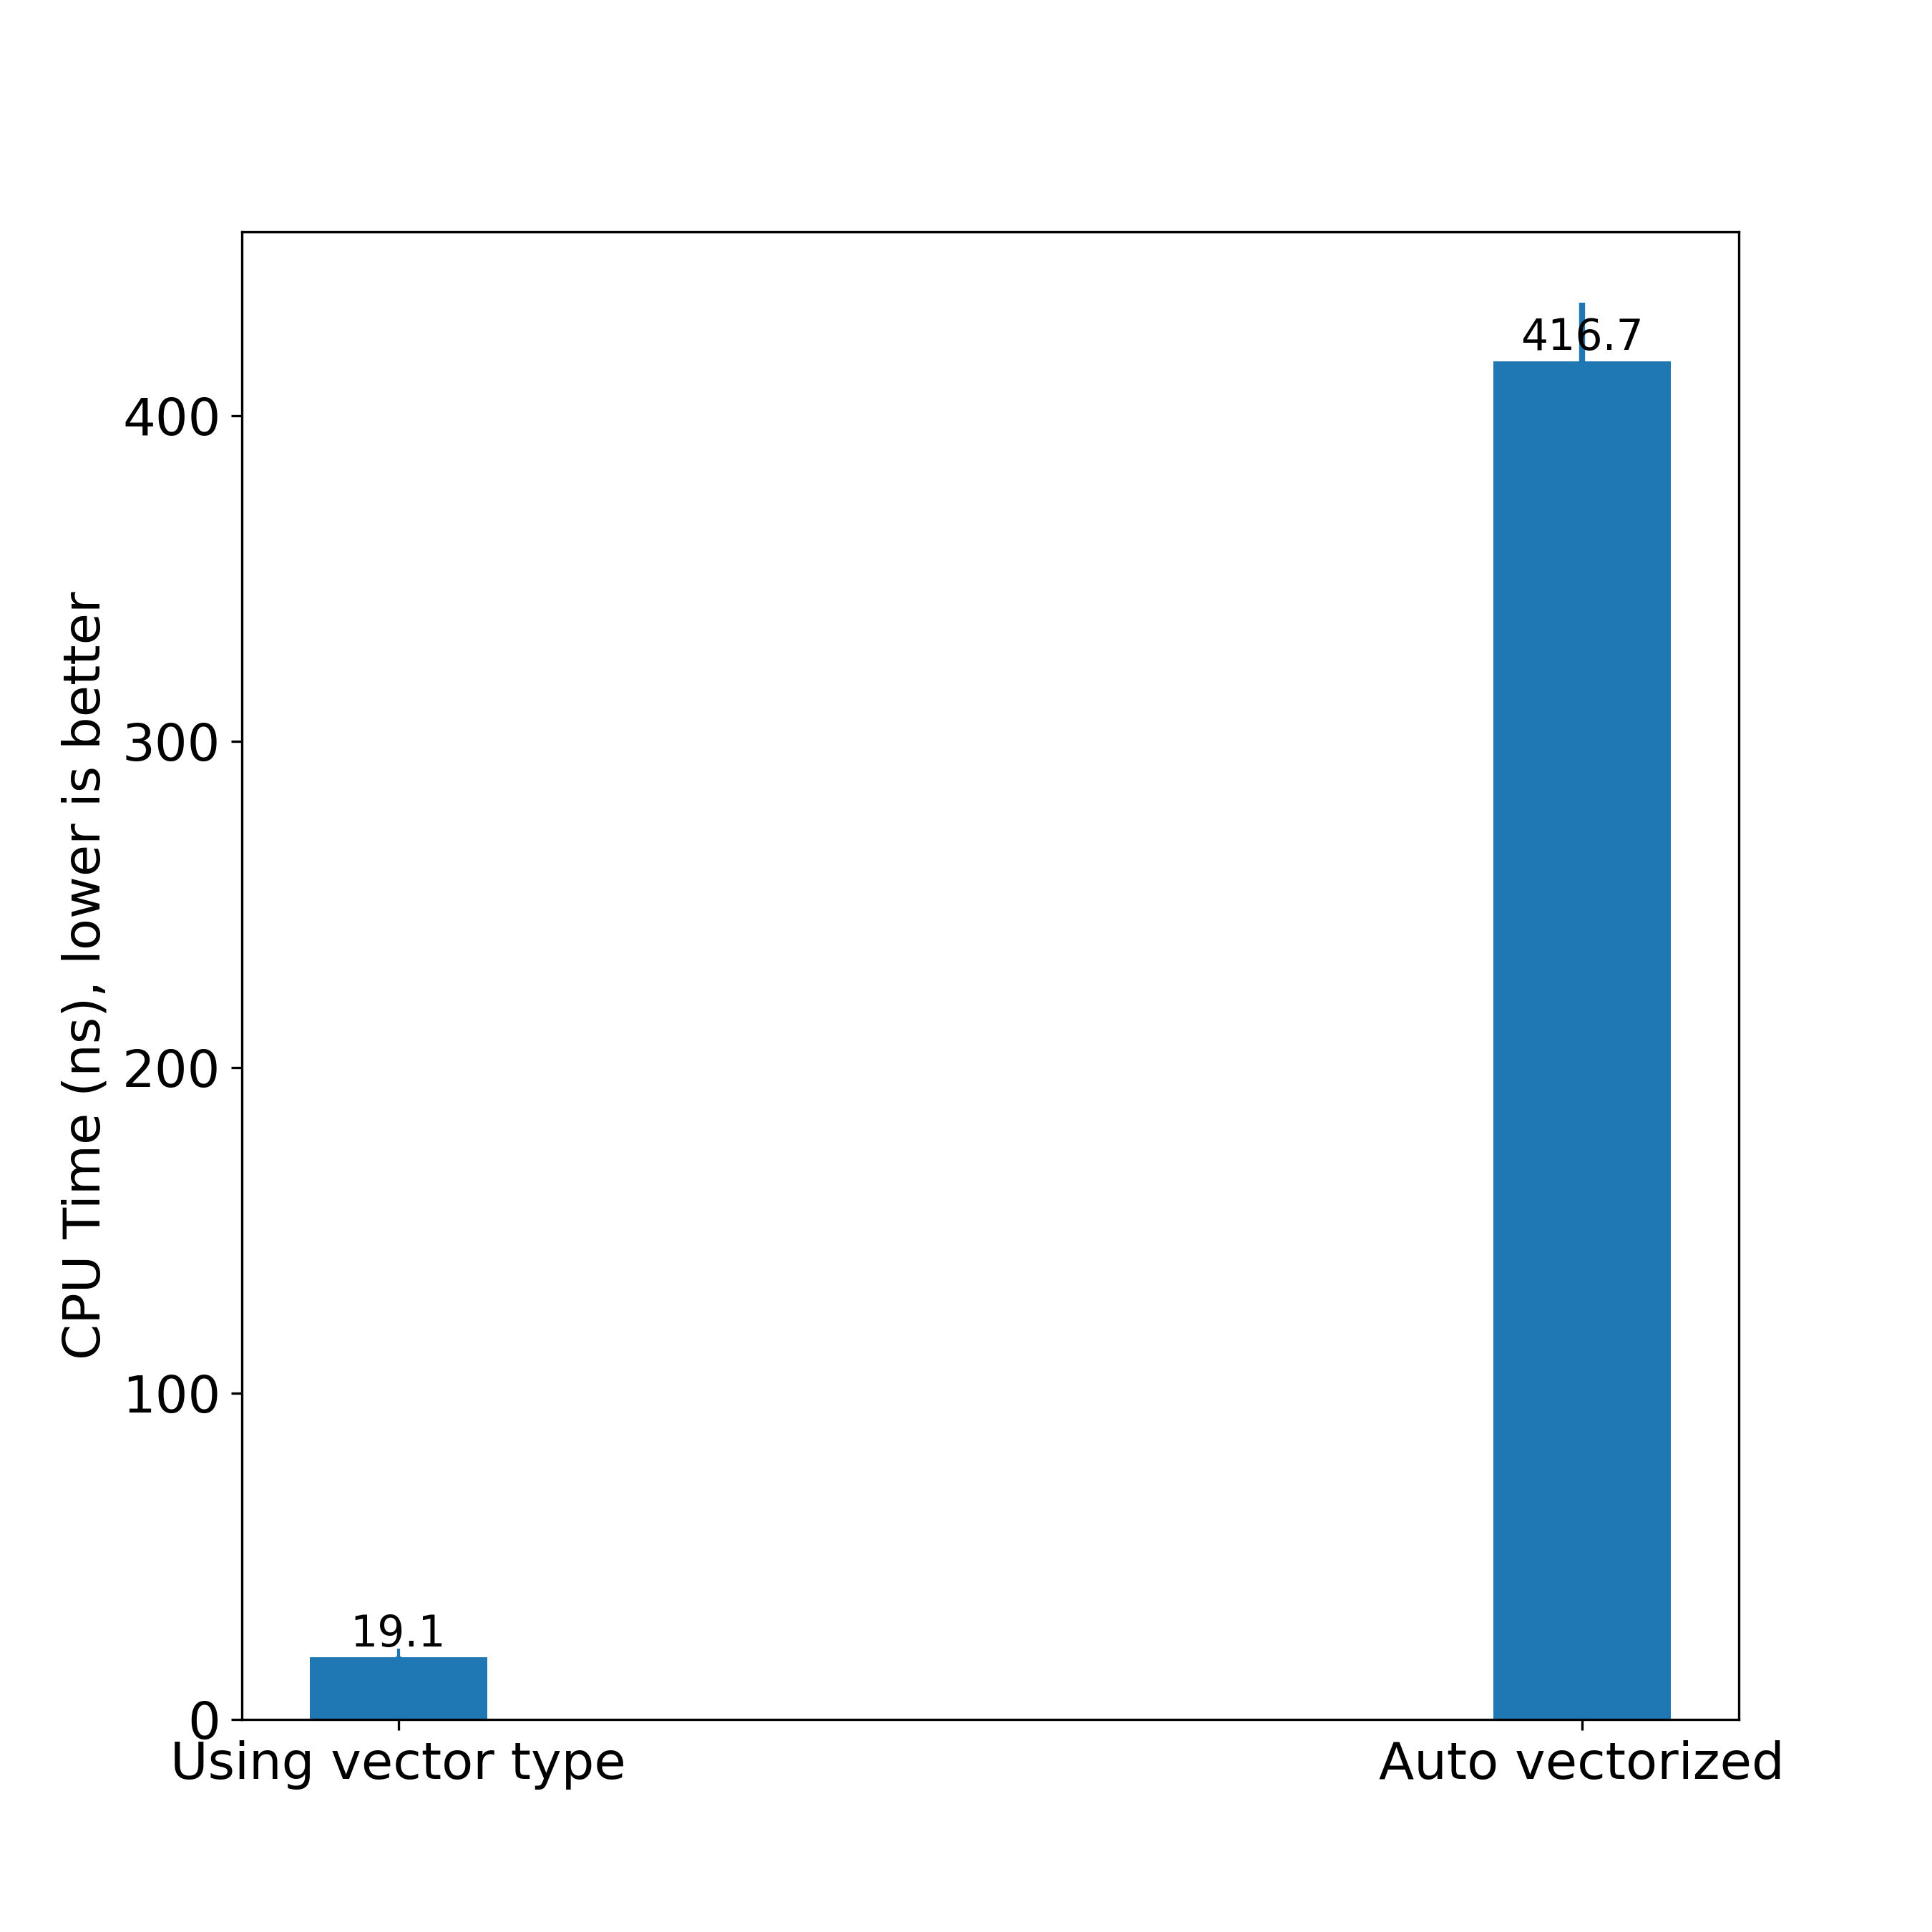
\includegraphics[width=\linewidth]{image/plot_vectorization_method.png}
    \end{center}
    \caption{A benchmark for the element-wise multiply-add toy example on 16
        by 16 matrices with different vectorization techniques. The toy example
        written with vector types is 5 to 10 times faster than their
        automatically vectorized or scalar counterpart. 
    % Also, \dtfloat{}
    % is always faster than \dtint{}, because it benefits from fused-multiply-add.
    }
    \label{plot_vectorization_method}
\end{figure}

    \begin{table}[H]\captionsetup{name=Listing}
%\captionsetup{justification=centering}
\begin{tabular}{>{\raggedright\arraybackslash}p{13cm}}
    Scalar source code to be automatically vectorized by Clang\\
    \midrule
    \begin{VerbatimCompact}
void vec_fma(matrix<int> & mat_src1, matrix<int> & mat_src2, 
             matrix<int> & mat_src3, matrix<int> & mat_dst) {
    for (int i = 0; i < row; i += 1) {
        for (int j = 0; j < col; j += 1) {
            int src1 = mat_src1.get(i,j);
            int src2 = ...
            mat_dst.set(i,j,  (src1 * src2) + src3);
        }
    }
}
    \end{VerbatimCompact}
    \\
    % \toprule
    Assembly snippet of the hot loop\\
    \midrule
    \begin{VerbatimCompact}
mov    0x1c(%rcx),%r13d
mov    0x1c(%rdx),%r12d
imul   %r14d,%r13d
imul   %r14d,%r12d
add    %r15d,%r13d
add    %r15d,%r12d
    \end{VerbatimCompact}
    \\
% \end{tabular}
% \caption{}
% \label{vec-fma-int-auto}
% \end{table}

% \begin{table}[H]\captionsetup{name=Listing}
% \begin{tabular}{>{\raggedright\arraybackslash}p{14cm}}

    Vectorized source code using Clang's vector type extension\\
    \midrule
    \begin{VerbatimCompact}
typedef int intZmm __attribute__((ext_vector_type(16)));
void vec_fma(matrix<int> & mat_src1, matrix<int> & mat_src2, 
             matrix<int> & mat_src3, matrix<int> & mat_dst) {
    int * src1_ptr = (int *) mat_src1.getItemPointer(0,0);
    int * src2_ptr = ...
    for (uint32_t i = 0; i < row * col; i += 16){
        intZmm src1Vec = *(intZmm *)(src1_ptr + i);
        intZmm src2Vec = *(intZmm *)(src2_ptr + i);
        intZmm src3Vec = *(intZmm *)(src3_ptr + i);
        *(intZmm *)(dst_ptr + i) = src1Vec * src2Vec + src3Vec;
    }
}
    \end{VerbatimCompact}
    \\
    % \toprule
    Assembly snippet of the hot loop\\
    \midrule
    \begin{VerbatimCompact}
vmovdqu64 (%rcx,%r8,4),%zmm0
vpmulld (%rax,%r8,4),%zmm0,%zmm0
vpaddd (%rsi,%r8,4),%zmm0,%zmm0
vmovdqu64 %zmm0,(%rdi,%r8,4)
    \end{VerbatimCompact}
    \\
\end{tabular}
\caption{Comparing to the source code from Listing \ref{table:vec-fma-float}, the
only change is replacing \dtfloat{} with \texttt{int}. Clang fails to vectorize the
scalar version, but vectorization is still successful with vector types. }
\label{vec-fma-int}
\end{table}





\section{Matrix Data Structure}
\label{sec:mat-structure}
The most intuitive data structure of a matrix is a nested list of lists, where each
list represents a row, and a list of rows is a matrix. In C++ this can be
represented using \texttt{std::vector<std::vector<T>>}, where \texttt{T} could
be \dtfloat{}, \dtdouble{}, \dtint{}, etc. The \texttt{std::vector}
class provides an intuitive interface for accessing and modifying elements,
making it easy to build a matrix data structure on top. 

One potential drawback of nested \texttt{std::vector} is that it requires two
indexing operations to access an element. An alternative implementation is to
“flatten” a matrix into a single \texttt{std::vector}, by simply concatenating
one row after another. To access a specific element, an index can be computed
manually using the given row and column: \texttt{column\char`_count * row + column}.
Compared to the list-of-lists approach, this reduces half of the memory indexing operation at the cost of extra
arithmetics. The differences between the two patterns are illustrated by an
example provided in Table \ref{table:nested-flat}. 

\begin{table}[ht]
%\captionsetup{justification=centering}
\begin{tabular}{%
    >{\raggedright\arraybackslash}p{2cm}%
    >{\raggedright\arraybackslash}p{6.5cm}%
    >{\raggedright\arraybackslash}p{4.5cm}}
    
    \toprule
    & Nested & Flat\\

    \midrule
    
    Type
    &
    \begin{VerbatimCompact}
std::vector<
    std::vector<int>>
    \end{VerbatimCompact}
    &
    \begin{VerbatimCompact}
std::vector<int>
    \end{VerbatimCompact}
    \\

Structure in Memory
    &
    \begin{VerbatimCompact}
vector of 4 = {
    vector of 4 = {0, 0, 0, 0}, 
    vector of 4 = {0, 0, 0, 0}, 
    vector of 4 = {0, 0, 0, 1}, 
    vector of 4 = {0, 0, 0, 0}
}
    \end{VerbatimCompact}
    &
    \begin{VerbatimCompact}
vector of 16 = {
    0, 0, 0, 0, 
    0, 0, 0, 0,
    0, 0, 0, 1, 
    0, 0, 0, 0
}
    \end{VerbatimCompact}
    \\

    Accessing row 2, column 3
    &
    Index row first: \texttt{std::vector<int>[2]} \linebreak
    then index column: 
        \texttt{std::vector<int>[2][3]}
    & 
    Compute \texttt{i = 
    \linebreak col\char`_count * row + col \linebreak = 4 * 2 + 3 =
    11}, \linebreak then index once: \texttt{std::vector<int>[11]}  \\

    \bottomrule

\end{tabular}
\caption{This is an example of a 4 by 4 matrix structured using nested and
flat lists, to highlight their differences.
}
\label{table:nested-flat}
\end{table}

Empirically indexing costs more time than integer multiplication and addition,
thus improving performance. Both the toy example and the \pivot{} function
perform sequential load-compute-store operations on each row and each column,
allowing the index of the next element to be computed by simply adding the step
% size or column size, further reducing memory overhead. In fact, 
% for element-wise matrix operations, such as the toy example or the \pivot{} function,
% % function can be optimized to only compute index once (See Section
% % \ref{sec:optmz-get-index}) by placing the pivot row as the first row. 
% it is only required to
% compute the address once for the first element of the matrix, and then every
% subsequent item can be indexed by address increments. 
Benchmark (Figure \ref{fig:nested-flat}) on the toy example confirms that for
16-row matrices with 16 column, 32 column or 64 column, the nested vector structure
is always about 8 ns slower than the flat matrix.

\begin{figure}
    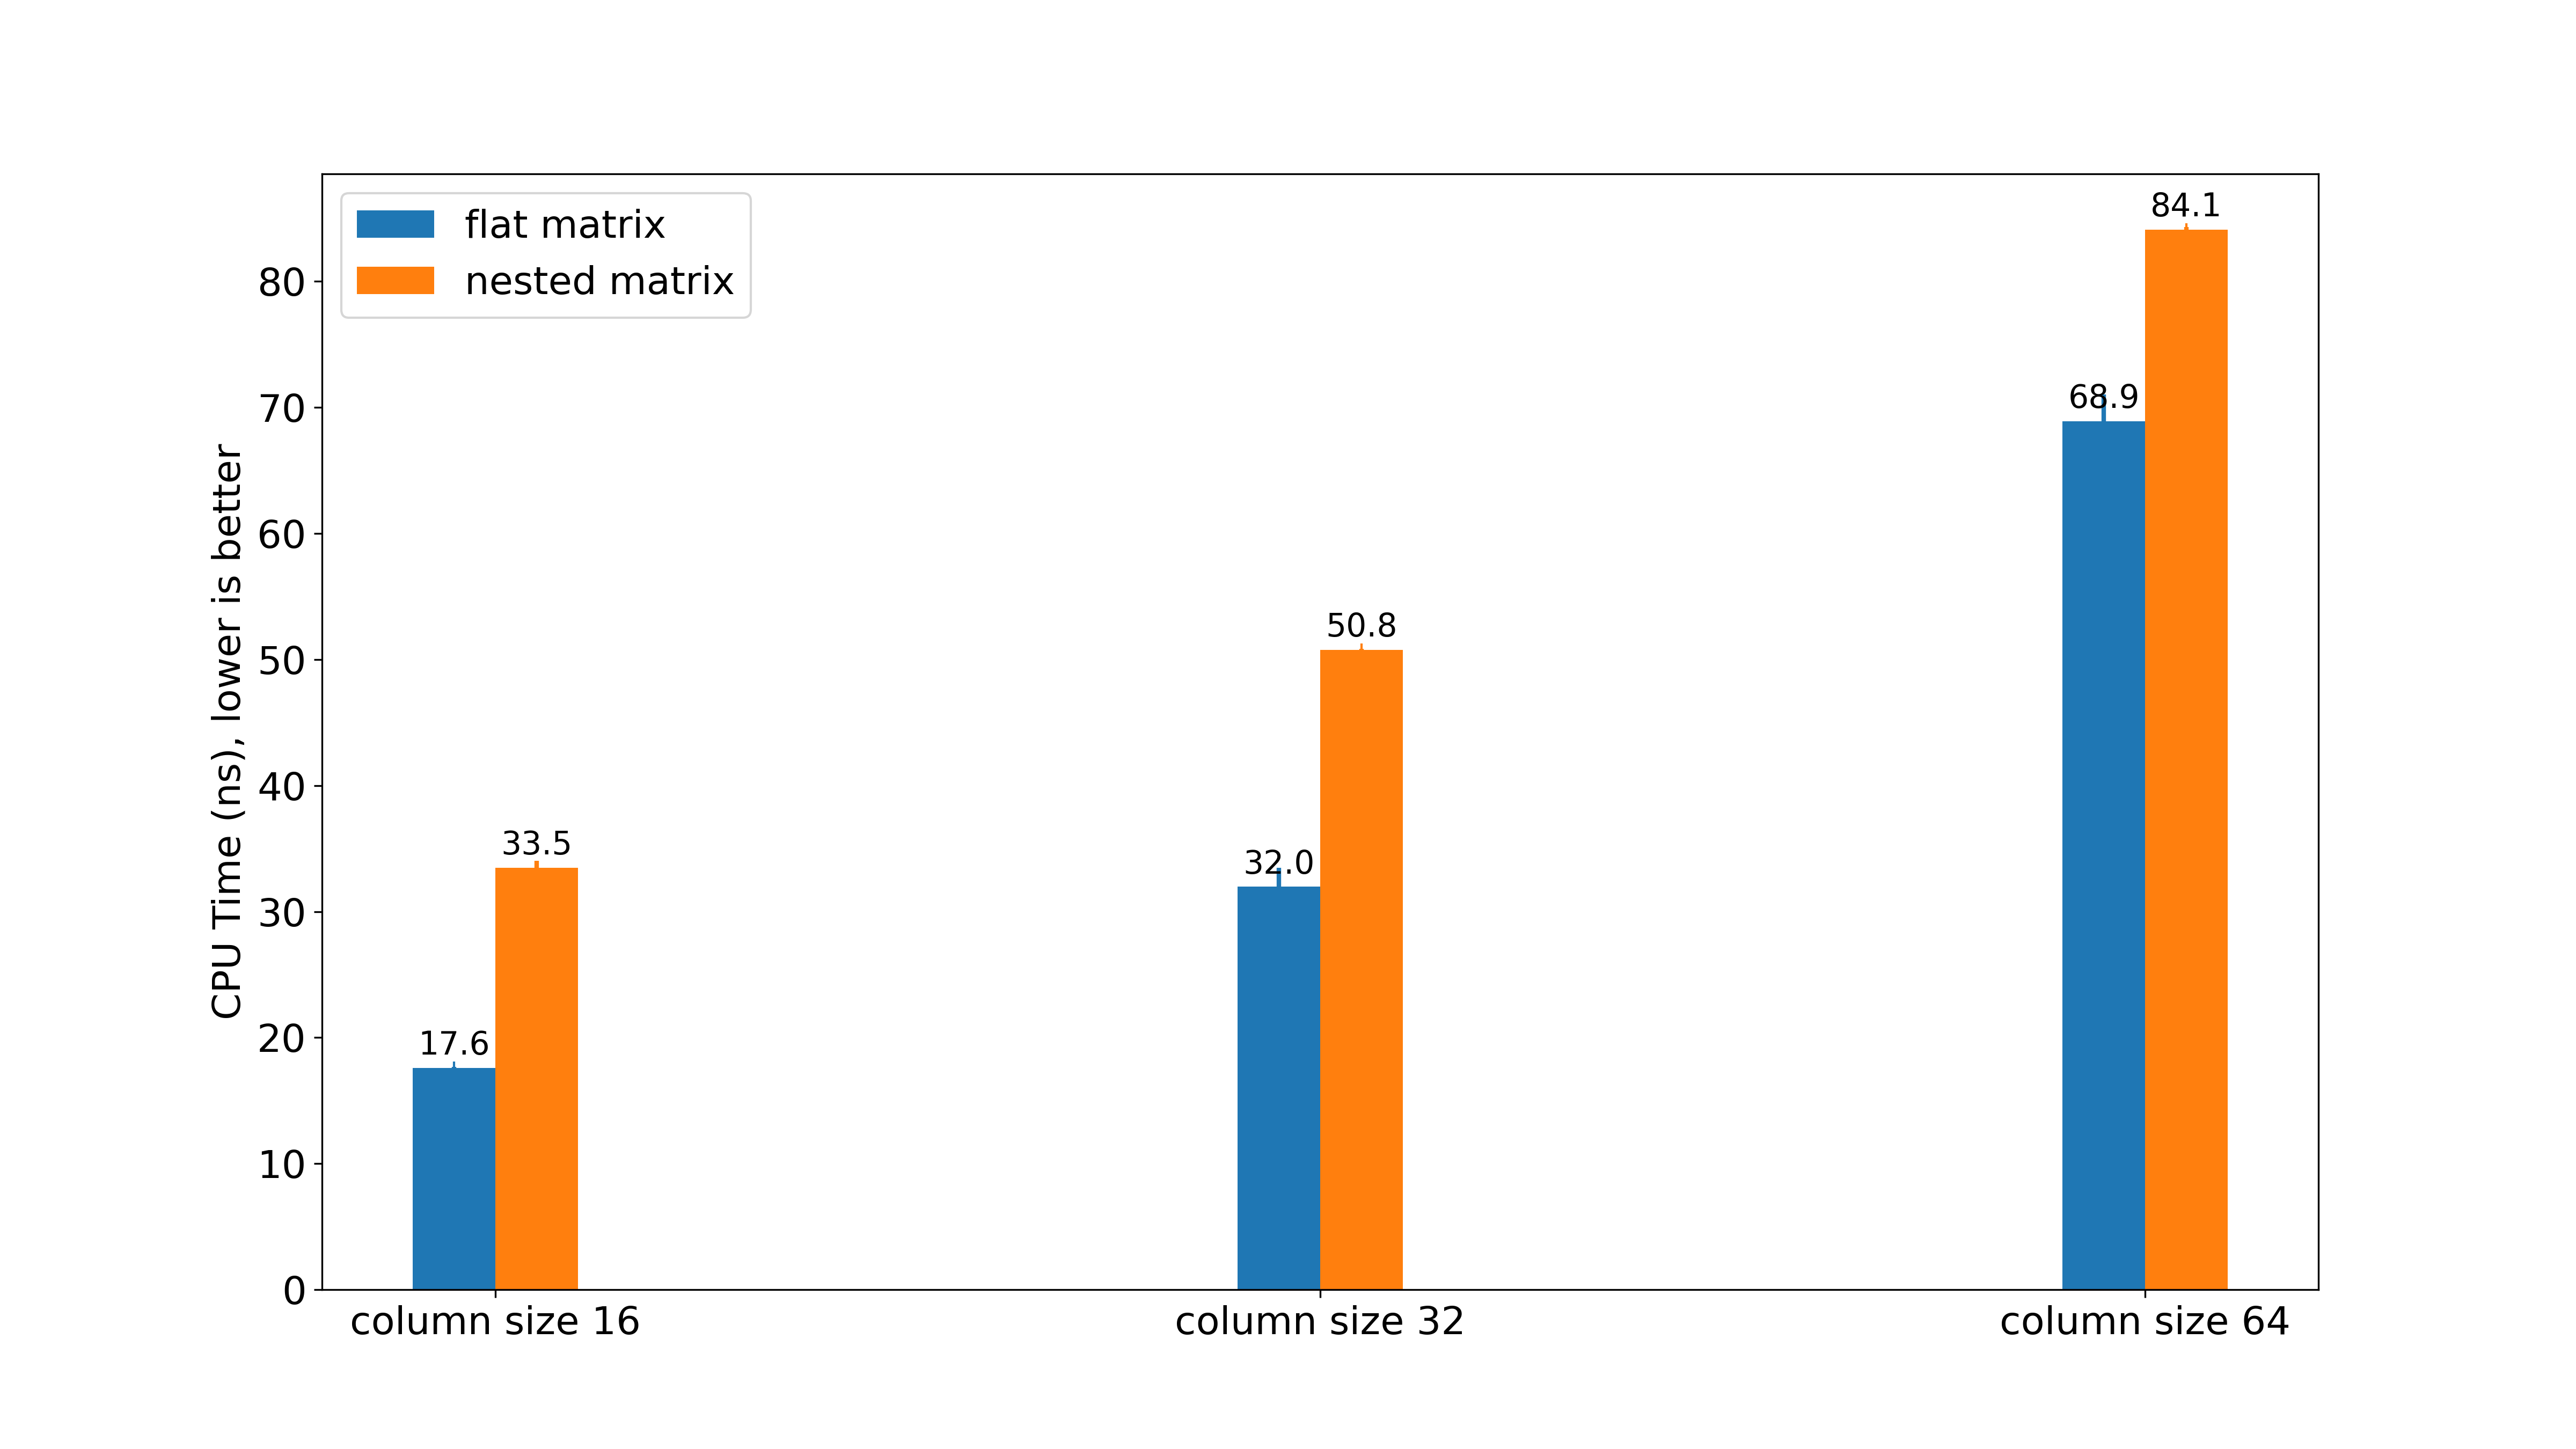
\includegraphics[width=\linewidth]{image/bench_nested_flat.png}
\caption{On a 16-row toy example doing \dtfloat{} FMA, selecting
the flat list as the data structure of the matrix is consistently faster than the
nested list implementation.  }
    \label{fig:nested-flat}
\end{figure}


\section{Matrix Element Data Type}


\subsection{Width}
\label{sec:width} 
Since the numbers stored in the matrix are almost always less than 10 bits,
using shorter data types can be more advantageous than longer ones because they
allow more numbers to be packed into a single vector register (Figure
\ref{archtable}). The number of instructions can be cut by half when the data width
is reduced to half, and less instruction count always leads to less execution
time. Given that the Zen 4 micro-architecture provides approximately the same amount
of execution units for both integers and floating points, it is reasonable to
estimate that the execution time is inversely proportional to the bit width of the
data type. As confirmed in Figure \ref{bench_datatype}, when overflow is
ignored, \dtint{} and \dtfloat{} cost nearly the same amount of time, while
\dtint{} and \dtdouble{} cost double the amount of time than \dtshort{} and
\dtfloat{} respectively.


\begin{figure}[H]\captionsetup{name=Figure}
    %\captionsetup{justification=centering}
    \begin{center}
        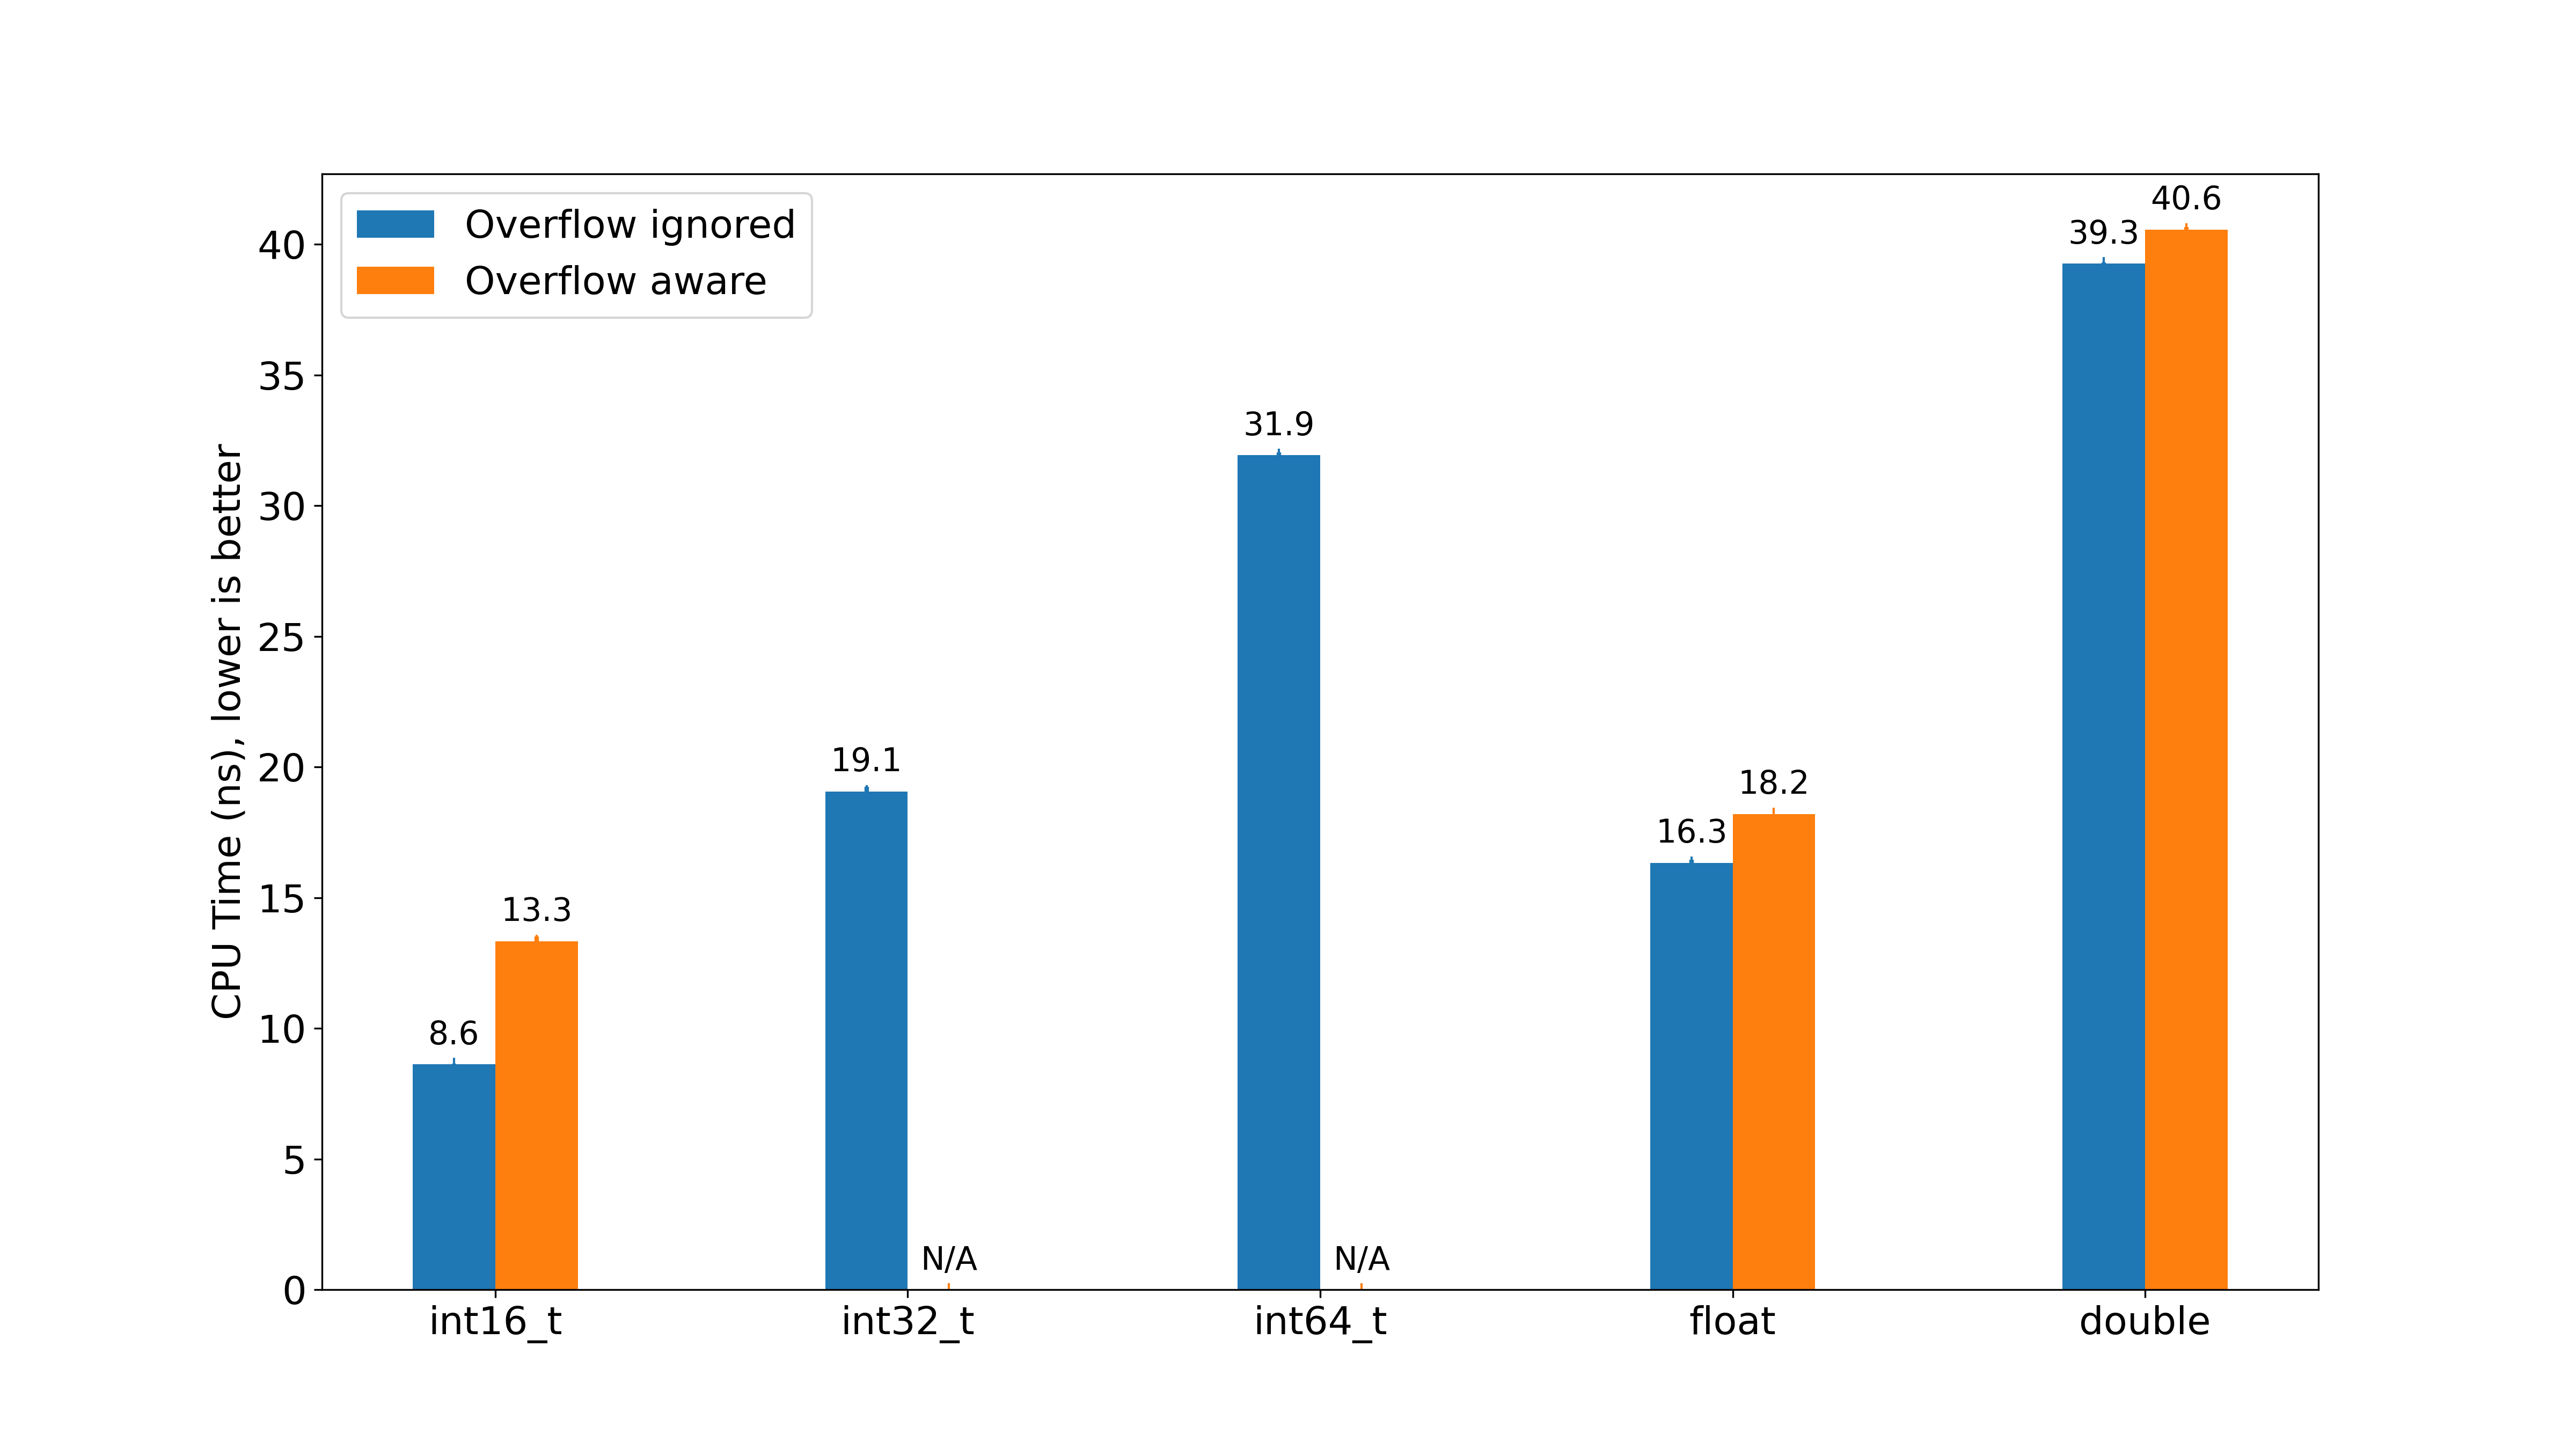
\includegraphics[width=\linewidth]{image/bench_datatype.png}
    \end{center}
    \caption{ A benchmark for toy example on a 16 by 16 matrix of \dtshort{},
\dtint{}, \dtlong{}, \dtfloat{}, and \dtdouble{}, with overflow checking turned
on or off. The runtime information for overflow checked \dtint{} and \dtlong{}
is not available, because it is difficult to implement vectorized overflow
checker. It is discovered that (1) runtime is
reduced by 50\% as the bit width of the data type is cut by half, (2) overflow
checking for integers is much more expensive than floating points. }
    \label{bench_datatype}
\end{figure}

% \begin{figure}[H]
%     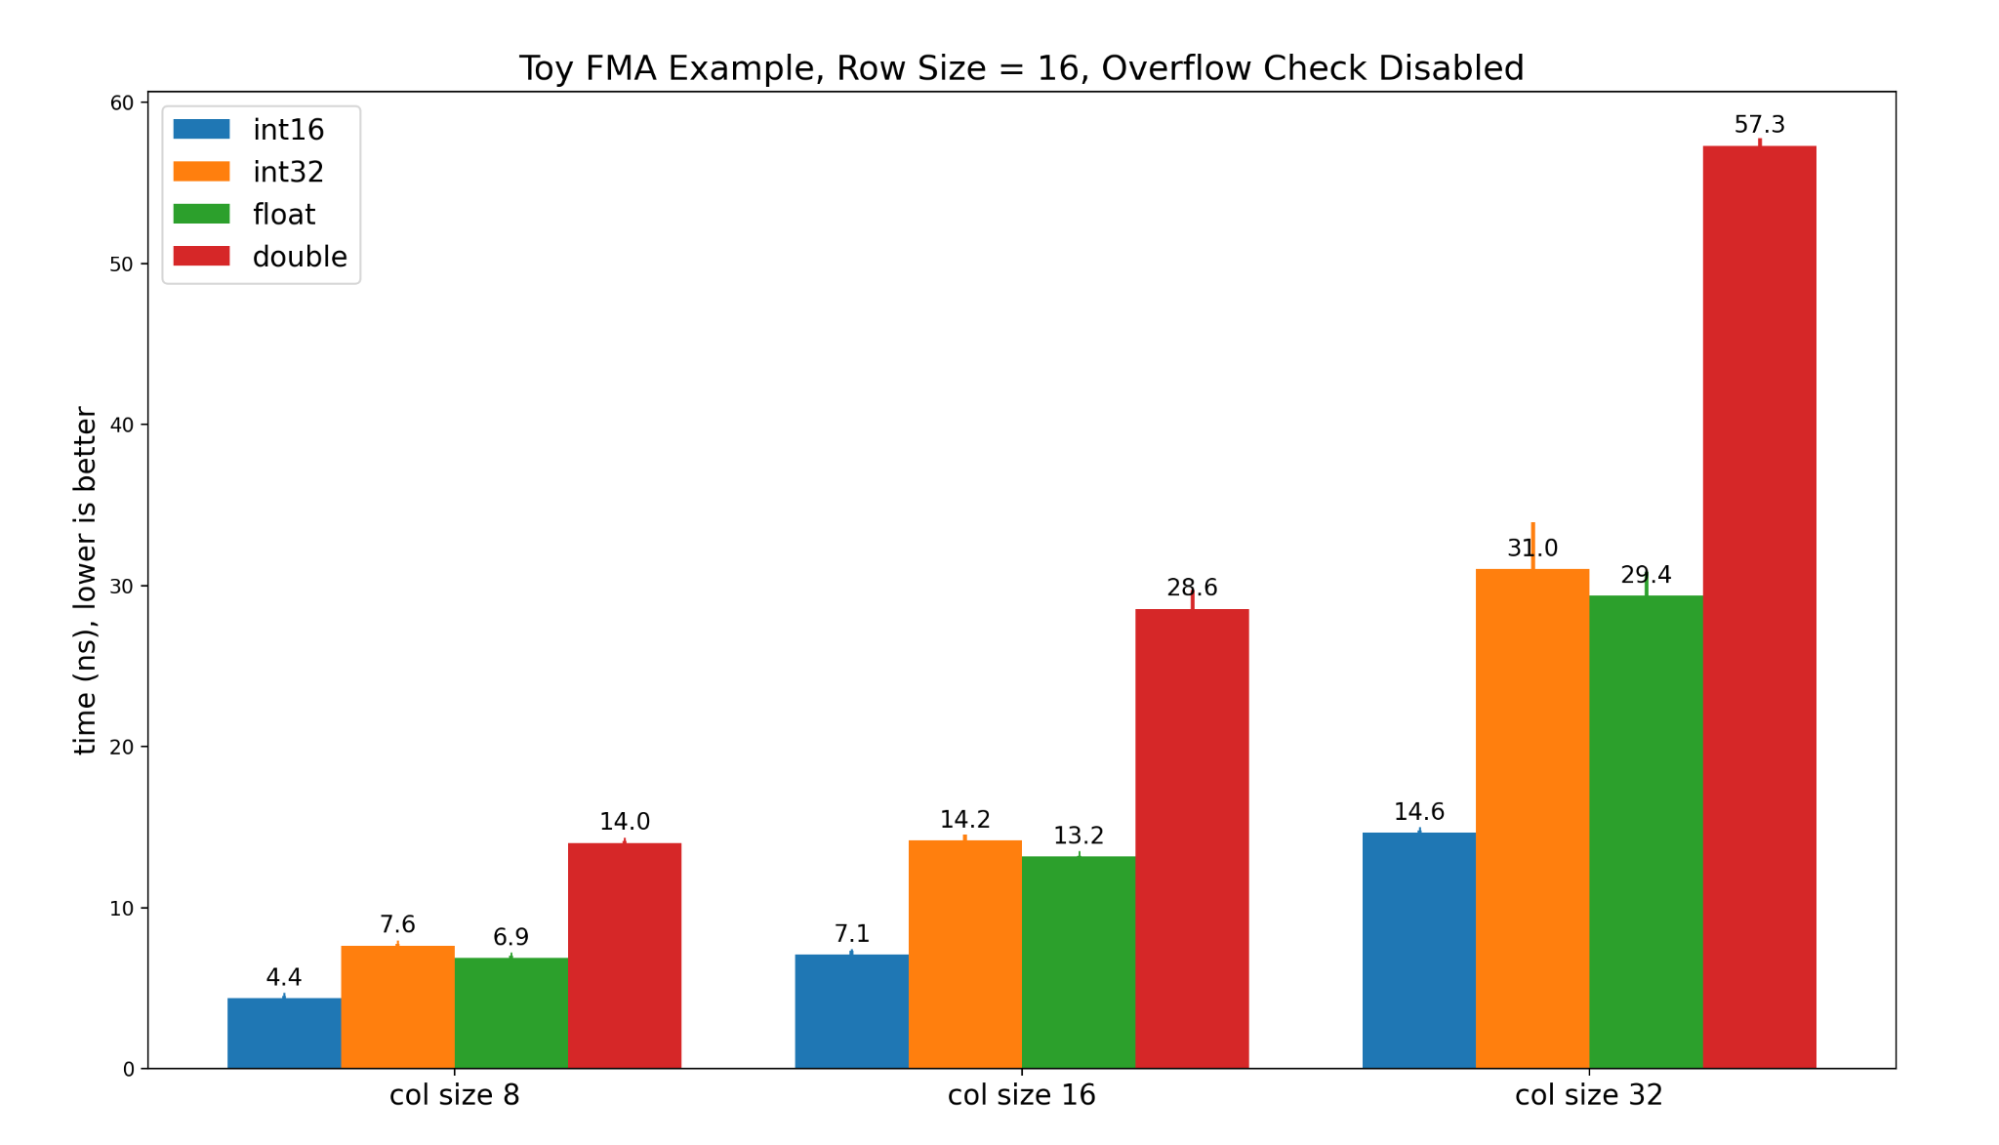
\includegraphics[width=\linewidth]{image/col8-col16-col32-i16-i32-f32-f64.png}
%     \caption{\hl{TODO: write caption}}
%     \label{fig:col8-col16-col32-i16-i32-f32-f64}
% \end{figure}

% \hl{TODO: fix Table number}
\begin{figure}[H]\captionsetup{name=Figure}
%\captionsetup{justification=centering}
    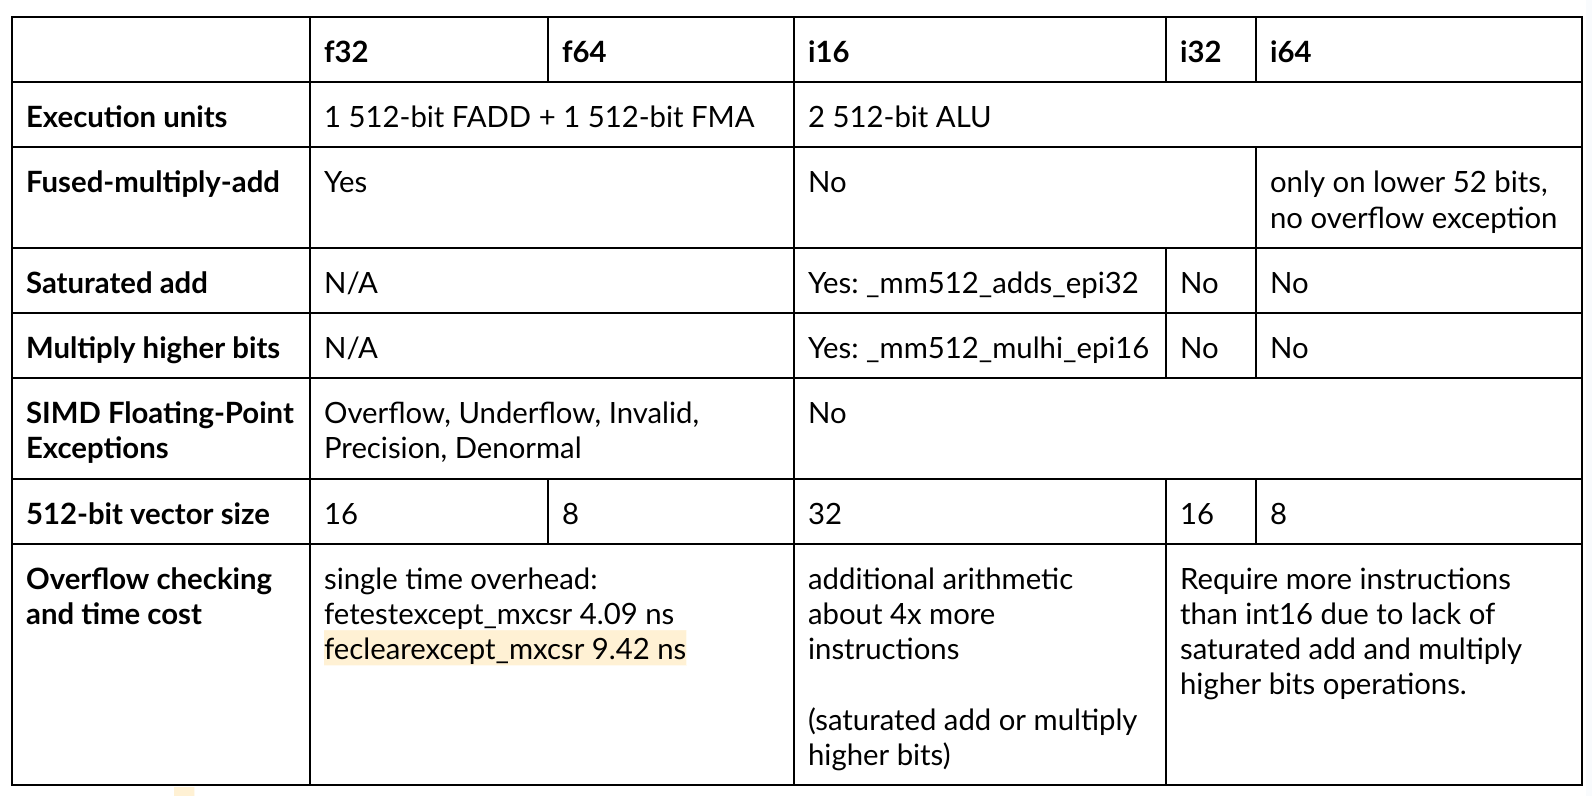
\includegraphics[width=\linewidth]{image/arch-table.png}
    \caption{A summary of features and resources provided by the Zen 4
    micro-architecture for different data
    types~\cite{Zen4Critique}~\cite{Zen2ChipWiki}.}
    \label{archtable}
\end{figure}

\subsection{Overflow Checking for Integers}
\label{sec:overflow-int}

The x86-64 micro-architecture provides the \texttt{seto} instruction to set some
byte to \texttt{1} if overflow occurred as a result of integer arithmetic.
However, \texttt{seto} only works for scalar operations. There is no instruction
or status register to indicate whether a previous vector add or multiply
instruction produced overflown results. Therefore, overflow has to be
checked manually by some additional vector instructions. This would slow down
the computation to some extent. Alternatively, arithmetics have to be
carried out on each element individually in a scalar manner, resulting in even
worse performance. 


% One advantage of using \dtshort{} is that it can be used with AVX-512's
% saturated add and multiply higher bits vector instructions, which are listed in
% Table \ref{archtable}. This allows for the creation of vectorized code that
% takes overflow into account and is therefore more efficient. However, it should
% be noted that there are no equivalent instructions for \texttt{int32_t} and
% \texttt{int64_t}.

One advantage of \dtshort{} is that it can be used with AVX-512's
saturated add and multiply higher bits vector instructions (Figure
\ref{archtable}), making it possible and convenient to write vectorized and
overflow-aware code. However, Zen 4's implementation of AVX-512
extension does not provide equivalent instruction for \dtint{} or \dtlong{} and
therefore must be processed as scalar values.
% When the
% result of a conventional add does not match the result of a saturated add, or
% when multiplying for the higher 16 bits gives non-zero results, it implies an
% overflow. 


\subsubsection{Implementation of Vectorized \dtshort{} Overflow Checking}
\label{sec:i16-overflow-checking}
By comparing the result of a conventional addition and saturated addition, it
indicates whether an addition has gone overflown or not. In case of overflow,
with saturated add, the result always retains at the maximum possible value of
\dtshort{}: \texttt{0x7FFF}, while the result of a conventional add is
always smaller because the overflowed output from conventional addition can't
go all the way around and become \texttt{INT16\char`_MAX} again. In the two's
complement binary form for integer, the overflow sum is "trapped" in the
negative number space. For example: 
\begin{verbatim}
INT16_MAX + 1 = INT16_MIN = -32768, 
INT16_MAX + 2 = -32767, 
...
INT16_MAX + INT16_MAX = -2, 
\end{verbatim}

For multiplication, two 16-bit numbers produce 32-bit products, but only lower 16
bits can be stored. Therefore, overflow can be detected by checking whether any
of the upper 16 bits are set. 

Inspecting these approaches from an instruction-level perspective (Table
\ref{table:i16-instr}), when overflow is ignored, both add and multiply takes 1
instruction, 
\hlc[pink]{\texttt{vpaddw}}\footnote{Vector add for \dtshort{}} 
and 
\hlc[pink]{\texttt{vpmullw}}\footnote{Vector multiply lower half bits for \dtshort{}}. 
To obtain and process overflow-related
information, an additional computation instruction
\hl{\texttt{vpaddsw}}\footnote{Vector saturated add for \dtshort{}}
or
\hl{\texttt{vpmulhw}}\footnote{Vector multiple higher half bits for \dtshort{}} 
is required, followed with 2 or 3 comparison, shuffling and branch instructions:
\hlc[cyan!60]{\texttt{vpsraw}}\footnote{Shift packed data right arithmetic},
\hlc[cyan!60]{\texttt{vpcmpneqw}}\footnote{Compare packed data for equal}
and 
\hlc[cyan!60]{\texttt{kord}}\footnote{Bitwise logical OR masks}. 
By enabling
overflow checking, it brings 4 to 5 times more instruction count and 65\% more
runtime~\cite{FPL2}.

\begin{center}
\begin{table}[ht]
\centering
%\captionsetup{justification=centering}
\begin{tabular}{  L{2cm}  L{5.5cm} L{5.5cm}  } 
     & Addition & Multiplication \\ 
    \midrule
        Overflow ignored 
    & 
        \hlc[pink]{\texttt{vpaddw \%zmm4,\%zmm2,\%zmm3}} 
    &
        \hlc[pink]{\texttt{vpmullw \%zmm1,\%zmm3,\%zmm2}} \\
    \midrule
        Overflow aware 
    &
        \hlc[pink]{\texttt{vpaddw \%zmm4,\%zmm2,\%zmm3}}
        \hl{\texttt{vpaddsw \%zmm2,\%zmm4,\%zmm2}}
        \hlc[cyan!60]{\texttt{vpcmpneqw \%zmm3,\%zmm2,\%k1}}
        \hlc[cyan!60]{\texttt{kord \%k1,\%k0,\%k0}}
    &  
        \hlc[pink]{\texttt{vpmullw \%zmm1,\%zmm3,\%zmm2}}
        \hl{\texttt{vpmulhw \%zmm1,\%zmm3,\%zmm3}}
        \hlc[cyan!60]{\texttt{vpsraw \$0xf,\%zmm2,\%zmm5}}
        \hlc[cyan!60]{\texttt{vpcmpneqw \%zmm3,\%zmm5,\%k1}}
        \hlc[cyan!60]{\texttt{kord \%k0,\%k1,\%k0}} \\
  \end{tabular}
\caption{This table highlights the difference in instruction count when
overflow checking is enabled or disabled for vectorized \dtshort{}.
\hlc[pink]{Pink} instructions are essential components as they compute the
anticipated arithmetic results, while overflow information are provided by
\hl{yellow} and \hlc[cyan!60]{cyan} instructions. }
  \label{table:i16-instr}
\end{table}
\end{center}
\subsubsection{Implementation of Scalar \dtint{} and \dtlong{}
Overflow Checking} 

Clang's language extension provides functions to perform overflow-checked
integer arithmetics: 
\begin{VerbatimCompact}
bool __builtin_add_overflow (type1 x, type2 y, type3 *sum);
bool __builtin_mul_overflow (type1 x, type2 y, type3 *prod);
\end{VerbatimCompact}
These functions take three arguments: \texttt{x} and \texttt{y} are the two
input operands, and \texttt{sum} or \texttt{prod} is a pointer to the variable
that will hold the result of the addition or multiplication. The return value of
these functions is a boolean that indicates whether an overflow occurred during
the operation. However, they do not accept vectors as input, and a loop around
these functions cannot be compiled into vector instructions either.


\subsection{Overflow Checking for Floating Points}
\label{sec:overflow-float}
To detect floating point overflow or imprecision, one approach is to enable
floating point imprecision as a trap, then upon overflow, the interrupt \sigfpe{}
is raised, and the PC (program counter) will be redirected to its handler. The
method can be programmed by using useful functions from the \texttt{fenv}
library as follow~\cite{fenvlib}:
\begin{verbatim}
void signal_handler(int signal) {
    // handle fpe
}

void function() {
    std::signal(SIGFPE, signal_handler);
    std::feclearexcept (FE_ALL_EXCEPT);
    feenableexcept (FE_INEXACT | FE_INVALID);
    // do something
    fedisableexcept (FE_INEXACT | FE_INVALID);
}
\end{verbatim}

In the \texttt{function()} block, first, the \texttt{std::signal()} function is
called to register the signal handler function for the \sigfpe{} interrupt. Next,
the \texttt{feclearexcept} function is called to clear any previously set
exception flags in the status register. Then, \feinexact{} and \feinvalid{} are
passed to the \texttt{feenableexcept()} function to enable inexactness and
invalid exceptions. Once the floating-point exceptions are enabled, 
computations can be performed. If some operation produces an inexact or invalid
floating point number, \sigfpe{} is raised, and a call to
\texttt{signal\char`_handler} is triggered. After the computation is completed,
the \texttt{fedisableexcept()} function is called to disable the previously
enabled exceptions. 

But it is difficult to recover back from \sigfpe{}. By design, the usage
of \sigfpe{} is to do some cleanup in the handler function, then exit the program
gracefully. If the handler does not exit the program after returning from the
handler, the PC always points back to the instruction that caused \sigfpe{} and
triggers \sigfpe{} again! However, the goal is to discard the current progress and
continue the program using the \texttt{LargeInteger}  algorithm. Although there could
be potential workarounds, such as modifying the call stack and changing the
return address, implementing these solutions can be challenging and
introduce significant complexity to the codebase.

Alternatively, we may read status registers and check if the imprecision bit is
set: 
\begin{verbatim}
bool function(matrix & tableau) {
    std::feclearexcept (FE_ALL_EXCEPT);
    if (fetestexcept(FE_INEXACT | FE_INVALID)) {
        // false for overflow, will be handle by its caller
        return false; 
    } return true; // true for safe
}
\end{verbatim}

Instead of registering floating point imprecision as interrupts, it clears the
floating point status register with \texttt{feclearexcept}. It reads the status
register afterwards using the \texttt{fetestexcept} function to check whether
imprecision has ever occurred in previous computations. It then returns a
boolean value to notify its caller whether or not the test for floating-point
exceptions is positive, \texttt{true} for safe and \texttt{false} for overflown.
In case of returning \texttt{false}, the caller will retry computation using
\texttt{LargeInteger} accordingly. 



\subsubsection{Evaluation}
In x86\_64 there are two status registers for floating points, the legacy x87
status register for traditional scalar floating point operation and the modern
\mxcsr{} register for SSE or AVX instructions. The source code
of the library function \texttt{fetestexcept} indeed manipulates both registers
\cite{fenvlib}: 
\begin{verbatim}
int fetestexcept(int excepts) {
    unsigned short status;
    unsigned int mxcsr;

    excepts &= FE_ALL_EXCEPT;

    /* Store the current x87 status register */
    __asm__ volatile ("fnstsw %0" : "=am" (status));

    /* Store the MXCSR register state */
    __asm__ volatile ("stmxcsr %0" : "=m" (mxcsr));

    return ((status | mxcsr) & excepts);
}
\end{verbatim}


In the vectorized floating point scenario, the instruction for the x87 status
register is unnecessary, and only the \mxcsr{} register should be concerned. The
hot loop is completely vectorized, and Clang dispatches 128-bit SSE
instructions for occasional scalar operations. The reason is that the SSE
execution units can handle both single and double precision floating point
arithmetic natively. In contrast, the legacy x87 floating-point instructions operate
on an 80-bit internal format, requiring additional conversions and delay. Using
SSE instructions reduce register pressure as well. The SSE
units have access to 16 \xmm{} registers, but for x87 units, only 8
floating point registers are available~\cite{x87-bad}. 

% . There could be even 32 \xmm{} registers if
% such an extension is implemented in the micro-architecture

As illustrated in Figure \ref{plot_fenv}, the benchmark evaluates the
performance of \texttt{fenv} functions alongside their respective revised
versions. The modifications involve restricting operations solely to
manipulating either the x87 status register or the \mxcsr{} register. It
indicates that it is significantly faster if we remove x87 status register
related operations. 

\begin{figure}[H]\captionsetup{name=Figure}
    %\captionsetup{justification=centering}
    \begin{center}
    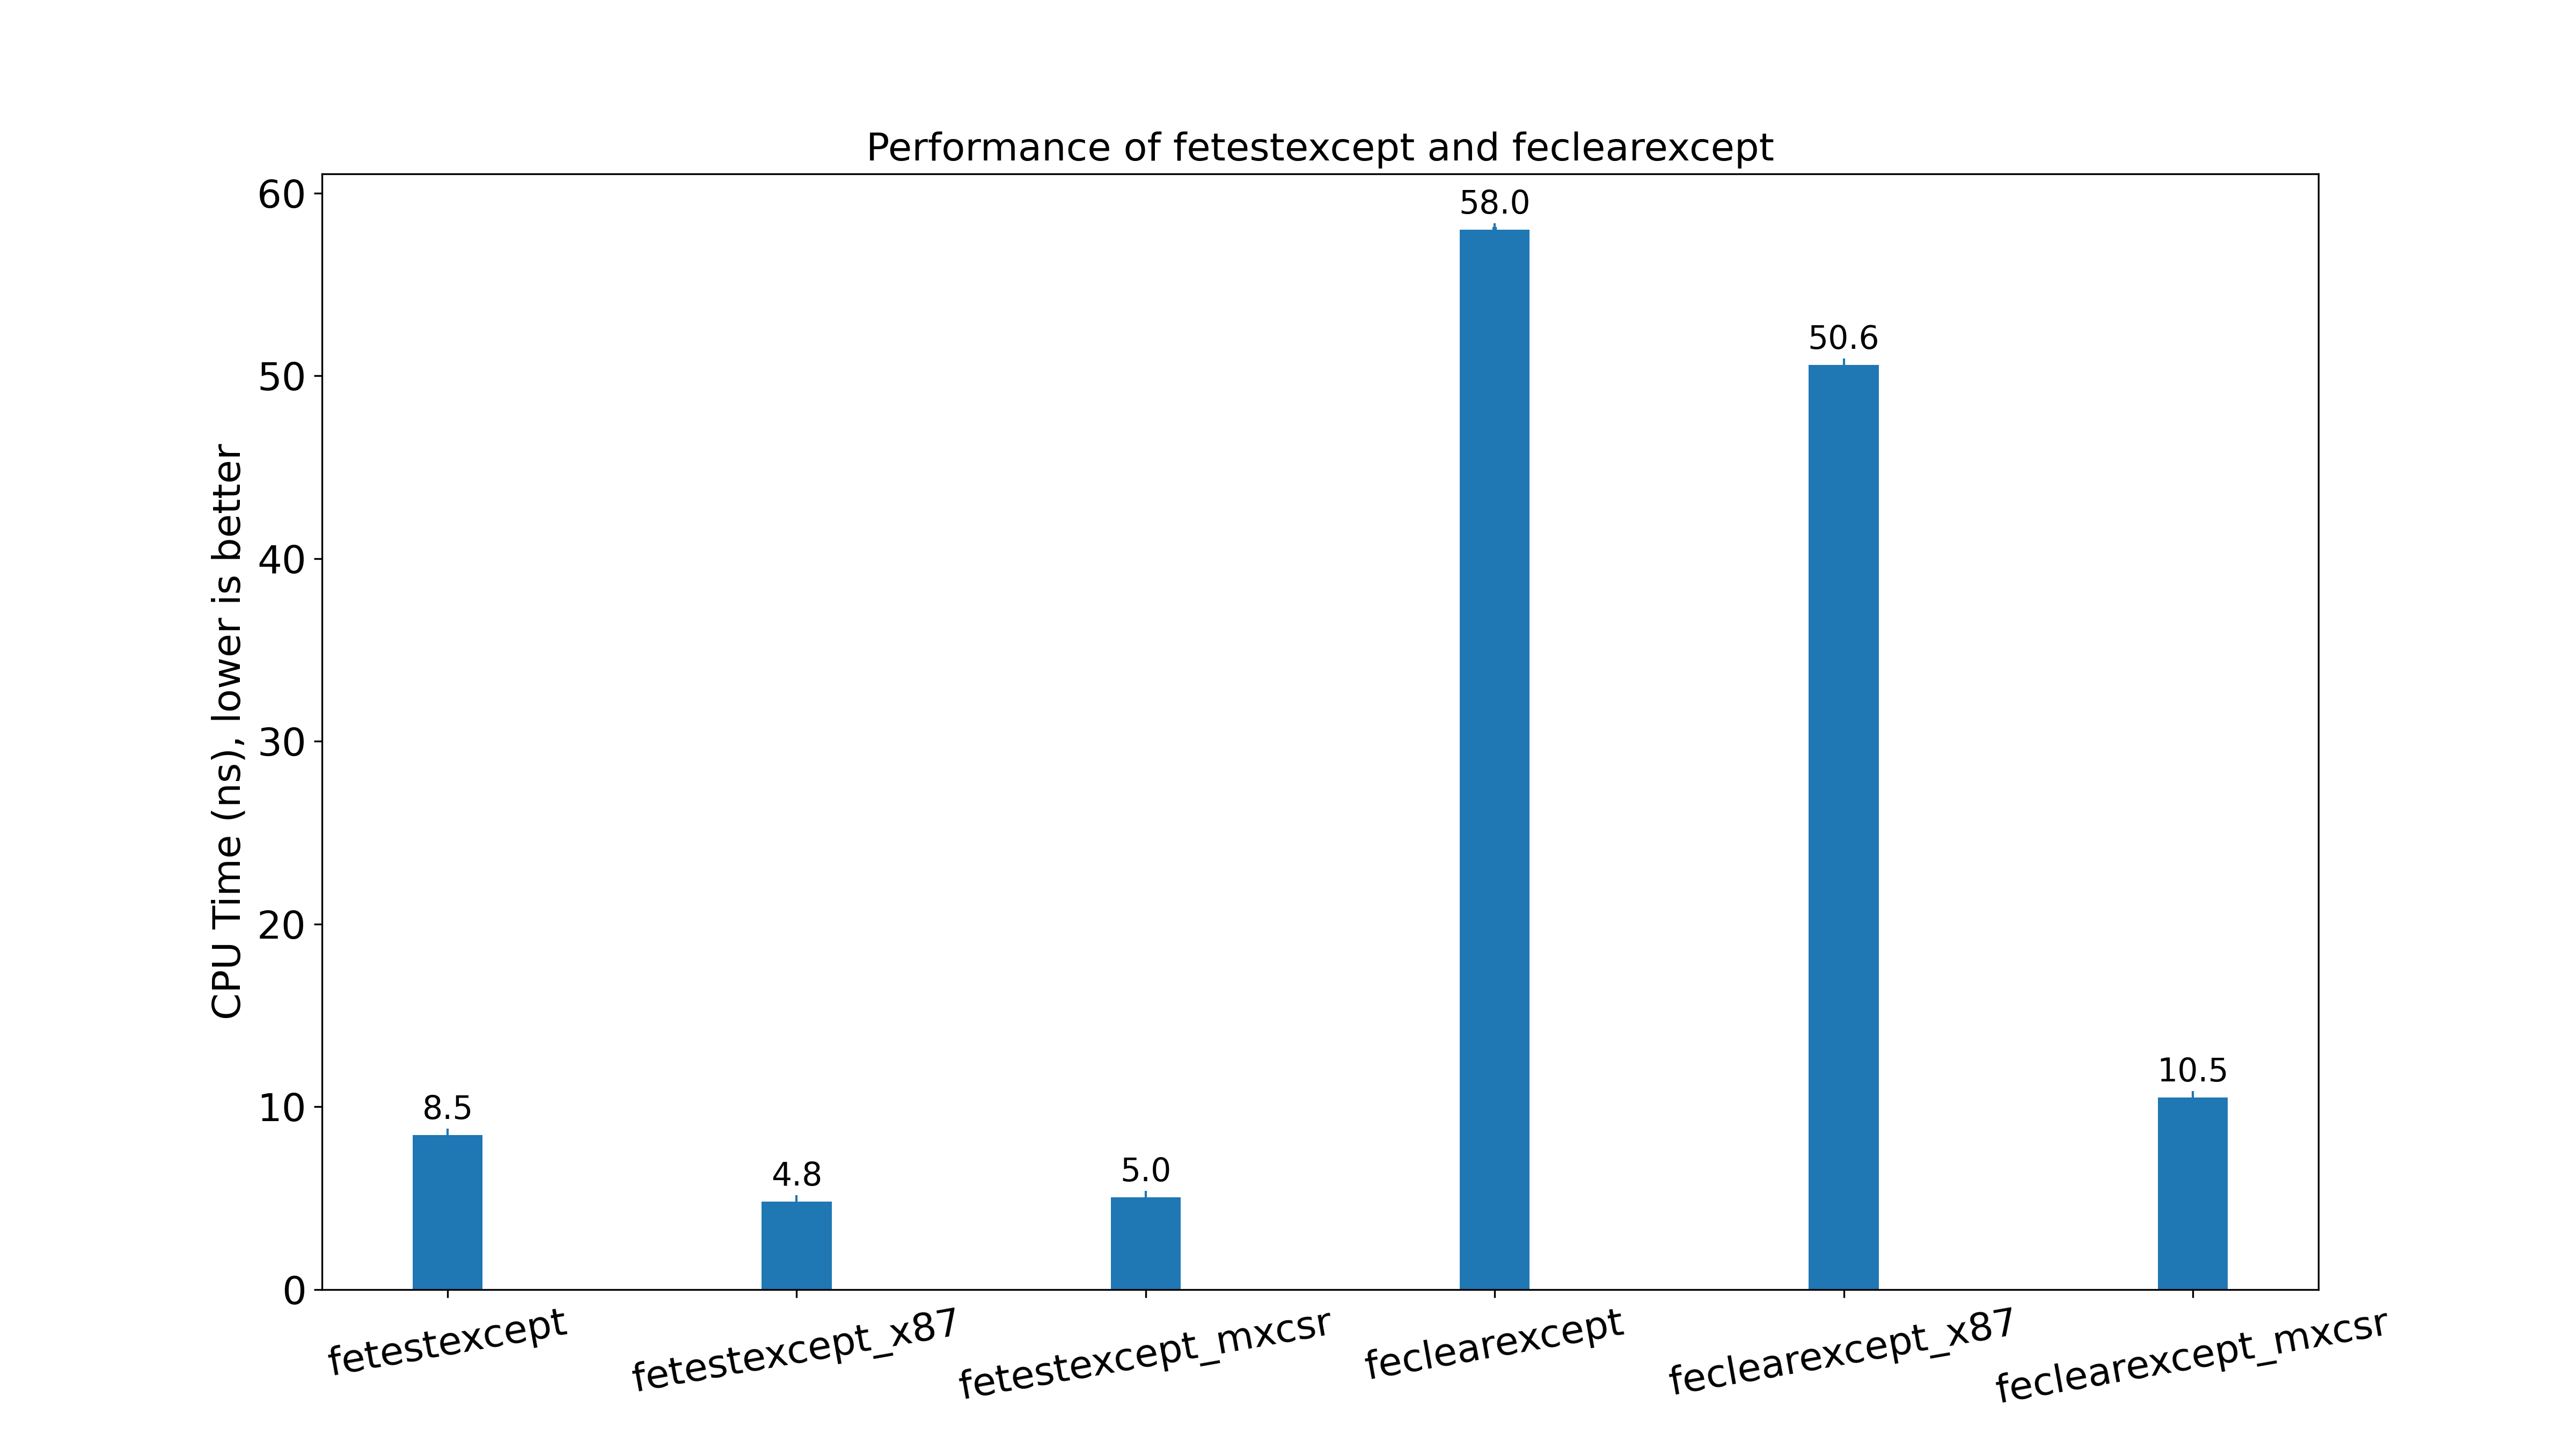
\includegraphics[width=\linewidth]{image/bench_fenv.png}
    \end{center}
    \caption{A benchmark for the floating point status register reading and
resetting functions from \texttt{cfenv} library and their modified versions that
only operate on either the x87 or the \mxcsr{} status register. Excluding x87
related operations makes both \texttt{fetestexcept} \texttt{feclearexcept}
faster.}
    \label{plot_fenv}
\end{figure}
\normalsize

\subsection{Comparing \dtshort{} and \dtfloat{}}

Section \ref{sec:width}, \ref{sec:overflow-int}, and \ref{sec:overflow-float}
have concluded that \dtshort{} is superior to any other integer data type and
\dtfloat{} is better than \dtdouble{}. 

% even
% though \dtshort{} is the fastest on this particular matrix size

Benchmark (Figure \ref{bench_datatype}) on the toy example reveals that
\dtshort{}'s spends a considerably higher percentage of runtime on overflow
checking compared with the floating point data types. This is consistent with
the reasoning from previous chapters, where overhead for \dtfloat{} is a
one-time expense, but for \dtshort{} it is always a portion of the total
runtime. 

Note that even though \dtshort{} is faster than \dtfloat{} in this benchmark, it is
not sound to conclude that the \pivot{} function implemented in \dtshort{} will be
faster than \dtfloat{}. The toy example is different from the \pivot{} function in
many aspects, for example, the number of memory load operations. In the actual
\pivot{} function, \dtfloat{} may potentially outperform \dtshort{}. 

% \begin{verbatim}
% bool function(matrix & tableau) {
%     // do something
%     if (fetestexcept(FE_INEXACT | FE_INVALID)) {
%     return false; // false for overflow, will be handle by its caller
%     } return true; // true for safe
% }

% void caller(){
%     ...
%     std::feclearexcept (FE_ALL_EXCEPT);
%     if (!function(tableau)) {
%         // overflow! retry with bigger precision algorithm
%     }
% }
% \end{verbatim}


\chapter{Implementation and Optimization of \pivot{}}
\label{sec:pivot-impl}
% \section{Overview}
The previous chapter on the top example have concluded that:
\begin{enumerate} 
    \item To achieve vectorization, source code should be written using Clang's
    vector type extension, rather than relying on compiler's automatic
    vectorizor. 
    \item Storing a matrix into a single flat list is more 
    advantageous than the nested list approach.
    \item The optimal integer and floating point data type is \dtshort{} and
    \dtfloat{} respectively. But it is difficult to tell
    which one is superior, because they have their own distinct advantages.
    \dtshort{} offers very short bit width, while \dtfloat{} provides quick overflow
    checking.
\end{enumerate}

After adopting clang's vector type and the flat list matrix design, this chapter
introduces some further optimizations to \pivot{} as the list below, and then
evaluates the performance of \pivot{} using either \dtshort{} or \dtfloat{} data
type.

\begin{enumerate} 
    \item Matrix-wise transprecision computing: minimizes the overhead
    of the transprecision dispatcher
    \item Double buffering: avoids the matrix being polluted by overflown data
    while not introduce additional memory copy operations. 
    \item Aligning the matrix to the size of vector registers: improves memory
    and cache IO utilization.
    \item Specialization for different row sizes: for \dtfloat{}, using 3 \ymm{}
    vectors for a row instead of 2 \zmm{} vectors reduces padding waste for each
    row and eliminates unnecessary arithmetic instructions.
\end{enumerate}


\section{Matrix-wise Transprecision}
Transprecision computing can be implemented at different levels of scale, such
as element-wise, row-wise, and matrix-wise (Figure
\ref{fig:transprecision-dispatch}). The transprecision dispatcher examining
overflow after computing on each element, each row or the entire matrix. If an
overflow occurs, the dispatcher interrupts its current progress, copies the 
matrix to fit a wider data type inside, then restarts dispatching using the wider
data type. 

\begin{figure}[H]
\begin{center}
    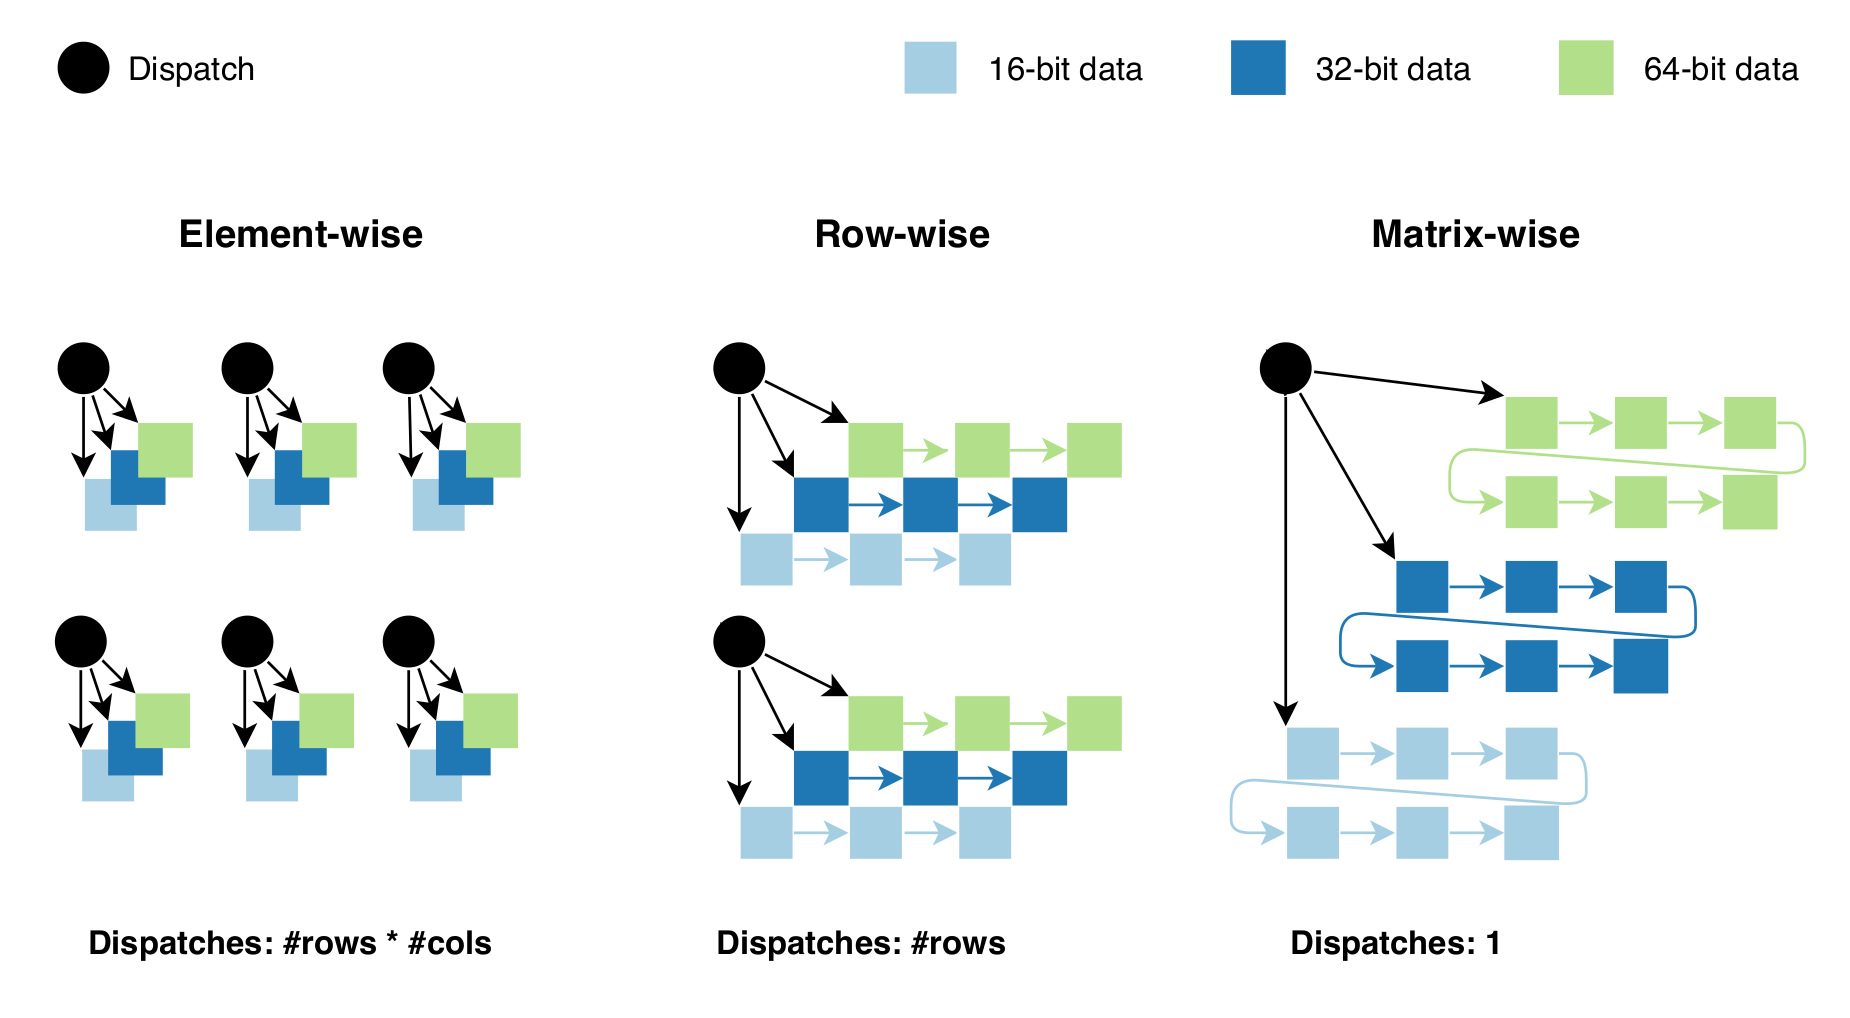
\includegraphics[width=\linewidth]{image/transprecision-dispatch.png}
    \caption{This figure illustrates how transprecision computing is organized
    from the perspective of the dispatcher. From row-wise to matrix-wise 
    transprecision, the cost of dispatching decreases \cite{FPL1}.}
    \label{fig:transprecision-dispatch}
\end{center}
\end{figure}
% For \dtfloat{}, the
% \mxcsr{} register accumulates information regarding previous overflow and
% imprecision occurrences until it is cleared manually. 

The \pivot{} function presented by this report is implemented using the
matrix-wise transprecision style, in order to minimize the runtime spent in the
dispatcher. The element-wise method is unsuitable in this scenario, as it
defeats the purpose of vectorization. The row-wise method is not chosen either,
due to that overflow is not likely to occur, and the matrix is small. Reading
the \mxcsr{} can be considered as an expensive operation compared to the time
spent on pivoting through the entire matrix. Avoid wasting runtime after
overflown at the cost of more \mxcsr{} reads is not a cost-effective
trade-off.

Even though the \pivot{} function using \dtshort{} was implemented using the
row-transprecision approach in previous works~\cite{FPL2}, it is modified to
match with the matrix-wise transprecision style to control differences
between the \dtfloat{} counterpart. After the overflow checking instructions,
instead of a branch instruction pointing to the overflow handler, the boolean
operator OR is applied between that overflow checking result register and an
overflow flag. 


\section{Double Buffering}

When matrix-wise computing is carried out, a potential overflow can contaminate
the input matrix and write meaningless results into it. It is difficult to
recover from overflown results, making it impossible to redispatch the same
input matrix to an algorithm of higher precision and defeating the purpose of
transprecision computing.

Double buffering (Figure \ref{fig:double-buffering}) 
addresses this problem of data pollution
caused by overflown data by allocating two pieces of
memory, one for the input matrix and the other for the output matrix. The input
matrix is read-only, while the output matrix allows read and write.
This separation of data storage ensures that the input matrix remains unpolluted
by overflown data and that any potential overflow is encapsulated within the
separate output matrix. 
\begin{figure}[H]
\centering
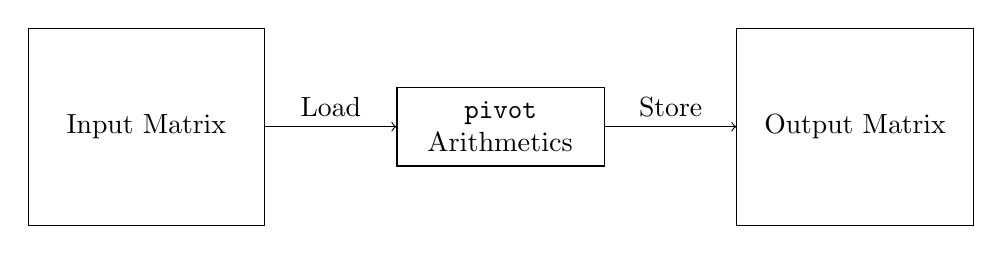
\begin{tikzpicture}[node distance=2cm]
    \node (buffer1) [rectangle, draw, minimum width=3cm, minimum height=2.5cm ] {Input Matrix};
    \node (compute) [rectangle, draw, text width=2.4cm, align=center, minimum width=1cm, minimum height=1cm, right of=buffer1, xshift=2.5cm] {\pivot{}\\Arithmetics};
    \node (buffer2) [rectangle, draw, minimum width=3cm, minimum height=2.5cm, right of=compute, xshift=2.5cm] {Output Matrix};

    \draw [->] (buffer1) -- node[above] {Load} (compute);
    \draw [->] (compute) -- node[above] {Store} (buffer2);
\end{tikzpicture}
\caption{The dataflow of the double buffered \pivot{}
function. Data is loaded from the input matrix, and stored to the output
matrix after computing.}
\label{fig:double-buffering}
\end{figure}


While making a copy of the input matrix (Figure \ref{fig:single-buffering}) 
is a simple and easy solution for
protecting the original data from pollution, double buffering is a superior
technique because it does not introduce additional memory operations. With
double buffering, every operand needs a load operation from the input matrix,
and every result takes a store operation to be written into the output matrix.
This is the minimal amount of memory operation required for arithmetics. Zen 4
can load one \zmm{} vector per cycle and store one \zmm{} vector per two
cycles. In comparison, it can do two multiplication or addition of \zmm{}
vectors every cycle~\cite{Zen4Critique}. The discrepancy in throughput between computing and IO
suggests that memory copy is very expensive and inefficient. 
\begin{figure}
\centering
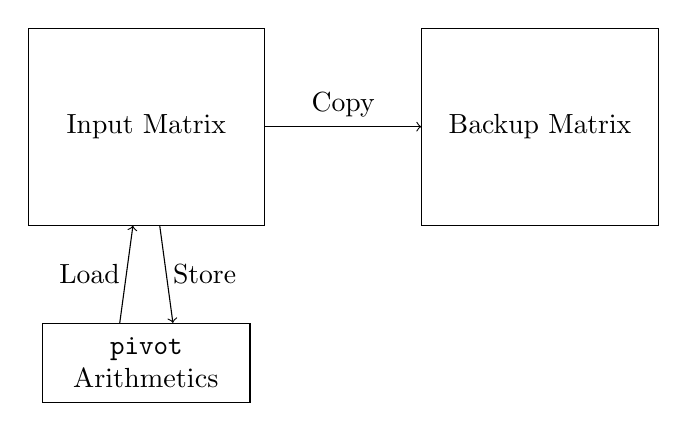
\begin{tikzpicture}[node distance=2cm]
    \node (buffer1) [rectangle, draw, minimum width=3cm, minimum height=2.5cm ] {Input Matrix};
    \node (buffer2) [rectangle, draw, minimum width=3cm, minimum height=2.5cm, right of=buffer1, xshift=3cm] {Backup Matrix};
    \draw [->] (buffer1) -- node[above] {Copy} (buffer2);
    
    \node (compute) [rectangle, draw, text width=2.4cm, align=center, minimum width=1cm, minimum height=1cm, below of=buffer1, yshift=-1cm] {\pivot{}\\Arithmetics};
    \draw [->] ([xshift=2cm]buffer1) -- node[left] {Load \phantom{11}} (compute);
    \draw [<-] ([xshift=-2cm]buffer1) -- node[right] {\phantom{51} Store} (compute);
\end{tikzpicture}
\caption{The dataflow of the \pivot{} function if it creates a
backup of the input matrix rather than double buffering. Comparing to 
Figure \ref{fig:double-buffering}, 
this method requires additional memory copy operations to make a backup.}
\label{fig:single-buffering}
\end{figure}


\section{Alignment}


The concept of memory alignment ensures that the starting address of each piece
of data is a multiple of its size. When accessing memory, the CPU retrieves data
from the main memory or cache in the unit of ``cache line'', and the cache lines
are aligned. Aligning the matrix to the size of vector registers guarantees that
every vector is fitted inside a single cache line. Otherwise, a vector register
might be spitted on two cache lines, then the CPU have to request both cache
lines and performs a shift to extract the desired vector~\cite{Unaligned}. A
simple example is provided by Figure \ref{fig:cacheline}.




% On Zen 4, the size of a
% cache line is 512 bits, precisely the size of a \zmm{}
% register~\cite{AMDManual}. 

In the Listing \ref{table:vec-fma-float} and Listing \ref{vec-fma-int}, the
assembly for load and store are \texttt{vmovups} and \texttt{vmovdqu64}.
\texttt{vmovups} for ``Move Unaligned Packed Single-Precision Floating-Point
Values'', and \texttt{vmovdqu64} for ``Move Unaligned Packed Integer
Values''~\cite{instruction}. This indicates that the load operation are unaligned,
and may bring negative impacts on performances~\cite{Unaligned}. 
To address this issue, an aligned allocator is given to the constructor of
\texttt{std::vector} when creating a matrix as follow, where the
\texttt{AlignedAllocator} is provided by the \dtshort{} implementation from the
FPL paper~\cite{FPL2}:
\begin{VerbatimCompact}
template <typename T>
class matrix {
public:
  std::vector<T, AlignedAllocator<T, 64>> m;
  // ...
}
\end{VerbatimCompact}
Loading from an aligned address can be noticed by the compiler, then aligned
load instructions \texttt{vmovdqa} or \texttt{vmovaps} will be selected
accordingly. 

\begin{figure} [H]
    \begin{center}
        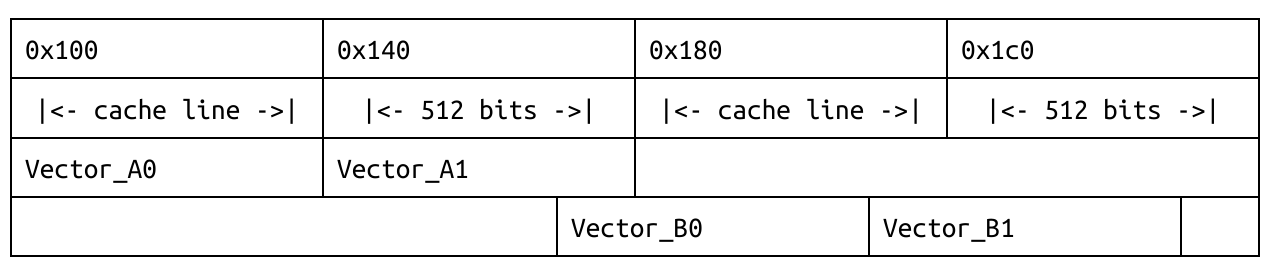
\includegraphics[width=\linewidth]{image/cacheline.png}
    \end{center}
    \caption{This example highlight the difference between 
    aligned loads and unaligned loads in the memory. 
    The vectors \texttt{Vector\char`_A*} are aligned 
    with the cache line size, loading them involves reading two of their 
    corresponding cache lines.
    However, \texttt{Vector\char`_B*}
    are unaligned, they are spitted on 3 cache lines. All 3 cache lines have to be
    read when loading the two \texttt{Vector\char`_B*} vectors. 
    }
    \label{fig:cacheline}
\end{figure}

% \section{Reduce Number of Matrix Index Computation}
% \label{sec:optmz-get-index}

% Section \ref{sec:mat-structure} discussed the benefits of using a single
% \texttt{std::vector} to represent a matrix. Given an arbitrary row and column,
% the item of the matrix can be found in the array by computing the index:
% \texttt{column\char`_count * row + column}. 
% By placing the pivot row as the
% first row in the matrix (Figure \ref{pivot-row-first}), it is only required to
% compute the address once for the first element of the matrix, and then every
% subsequent item can be indexed by address increments. 


% % The matrix data structure can be further
% % optimized if the number of index computations can be reduced.



% \begin{table}[H]
% \begin{minipage}{.5\linewidth}
% \begin{tabular}{|l|l|}
% \hline
% Row        & Content \\ 
% \toprule
% $0$    & First row of the matrix \\ 
% \phantom{} &                         \\
% ...        &  ...                    \\
% \phantom{} &                         \\
% $p-1$   & The row before pivot row  \\ 
% \hline
% $p$  & \tikz[baseline=(node1.base)]\node (node1)  {\textbf{Pivot row}};    \\ 
% \hline
% $p+1$   & The row after pivot row  \\ 
% \phantom{} &                         \\
% ...        &  ...                    \\
% \phantom{} &                         \\
% $n-1$    & Last row of the matrix \\ 
% \hline
% \end{tabular}

% \end{minipage}%
% \begin{minipage}{.5\linewidth}

% \begin{tabular}{|l|l|}
% \hline
% Row        & Content \\ 
% \toprule
% $0$  &   \tikz[baseline=(node2.base)]\node (node2) {\textbf{Pivot row}};  \\ 
% \hline
% $1$        & First row of the matrix \\ 
% \phantom{} &                         \\
% ...        &  ...                    \\
% \phantom{} &                         \\
% $p-1$   & The row before pivot row  \\ 
% $p$   & The row after pivot row  \\ 
% \phantom{} &                         \\
% ...        &  ...                    \\
% \phantom{} &                         \\
% $n-1$    & Last row of the matrix \\ 
% \hline
% \end{tabular}
% \end{minipage} 

% % \begin{tikzpicture}[remember picture,overlay]
%     % % Bend above text line
%     % \draw[-latex] (node2.south) -- ++(0,-1.5ex) -| (node1.south);
%     % % \draw[-latex] (node2.north) to[bend right] (node1.north);
% % \end{tikzpicture}

% \caption{The tables highlight the difference between two different approaches in
% arranging rows of a $n$-row matrix in the memory. The left-hand-side presents
% the structure of the matrix by default, while the matrix on the right is derived
% by moving the pivot row to the first row of the matrix.}
% \label{pivot-row-first}
% \end{table}



\section{Column Size Specialization}
\label{sec:ColumnSizeSpecialization}

A single \zmm{} vector can accommodate up to 16 \dtfloat{} values, while two of
them can store 32 \dtfloat{} values. However, loading a row into two \zmm{}
vectors can result in a minimum waste of 12 \dtfloat{} values for 95\% of
matrices containing 20 columns or less, as indicated in Figure
\ref{small-val-low-dim}. Alternatively, rows can be into loaded into multiple
\ymm{} vectors, which can accommodate 8 \dtfloat{} values each. For the majority
of cases, 3 \ymm{} vectors can sufficiently cover the aforementioned 95\% of
matrices with substantially less waste. Since \ymm{} registers have double the
amount of execution units than \zmm{}, and the instruction count is anticipated
to be only 50\% greater, the use of a 3 \ymm{} setup for a row is expected to
outperform the 2 \zmm{} approach. Benchmark plotted in the Figure
\ref{fig:3ymm-4ymm-2zmm} demonstrates that the 3 \ymm{} setup for a row is 15\%
faster then the 2 \zmm{} configuration, which matches the expectation.

\begin{figure}[H]
    \begin{center}
        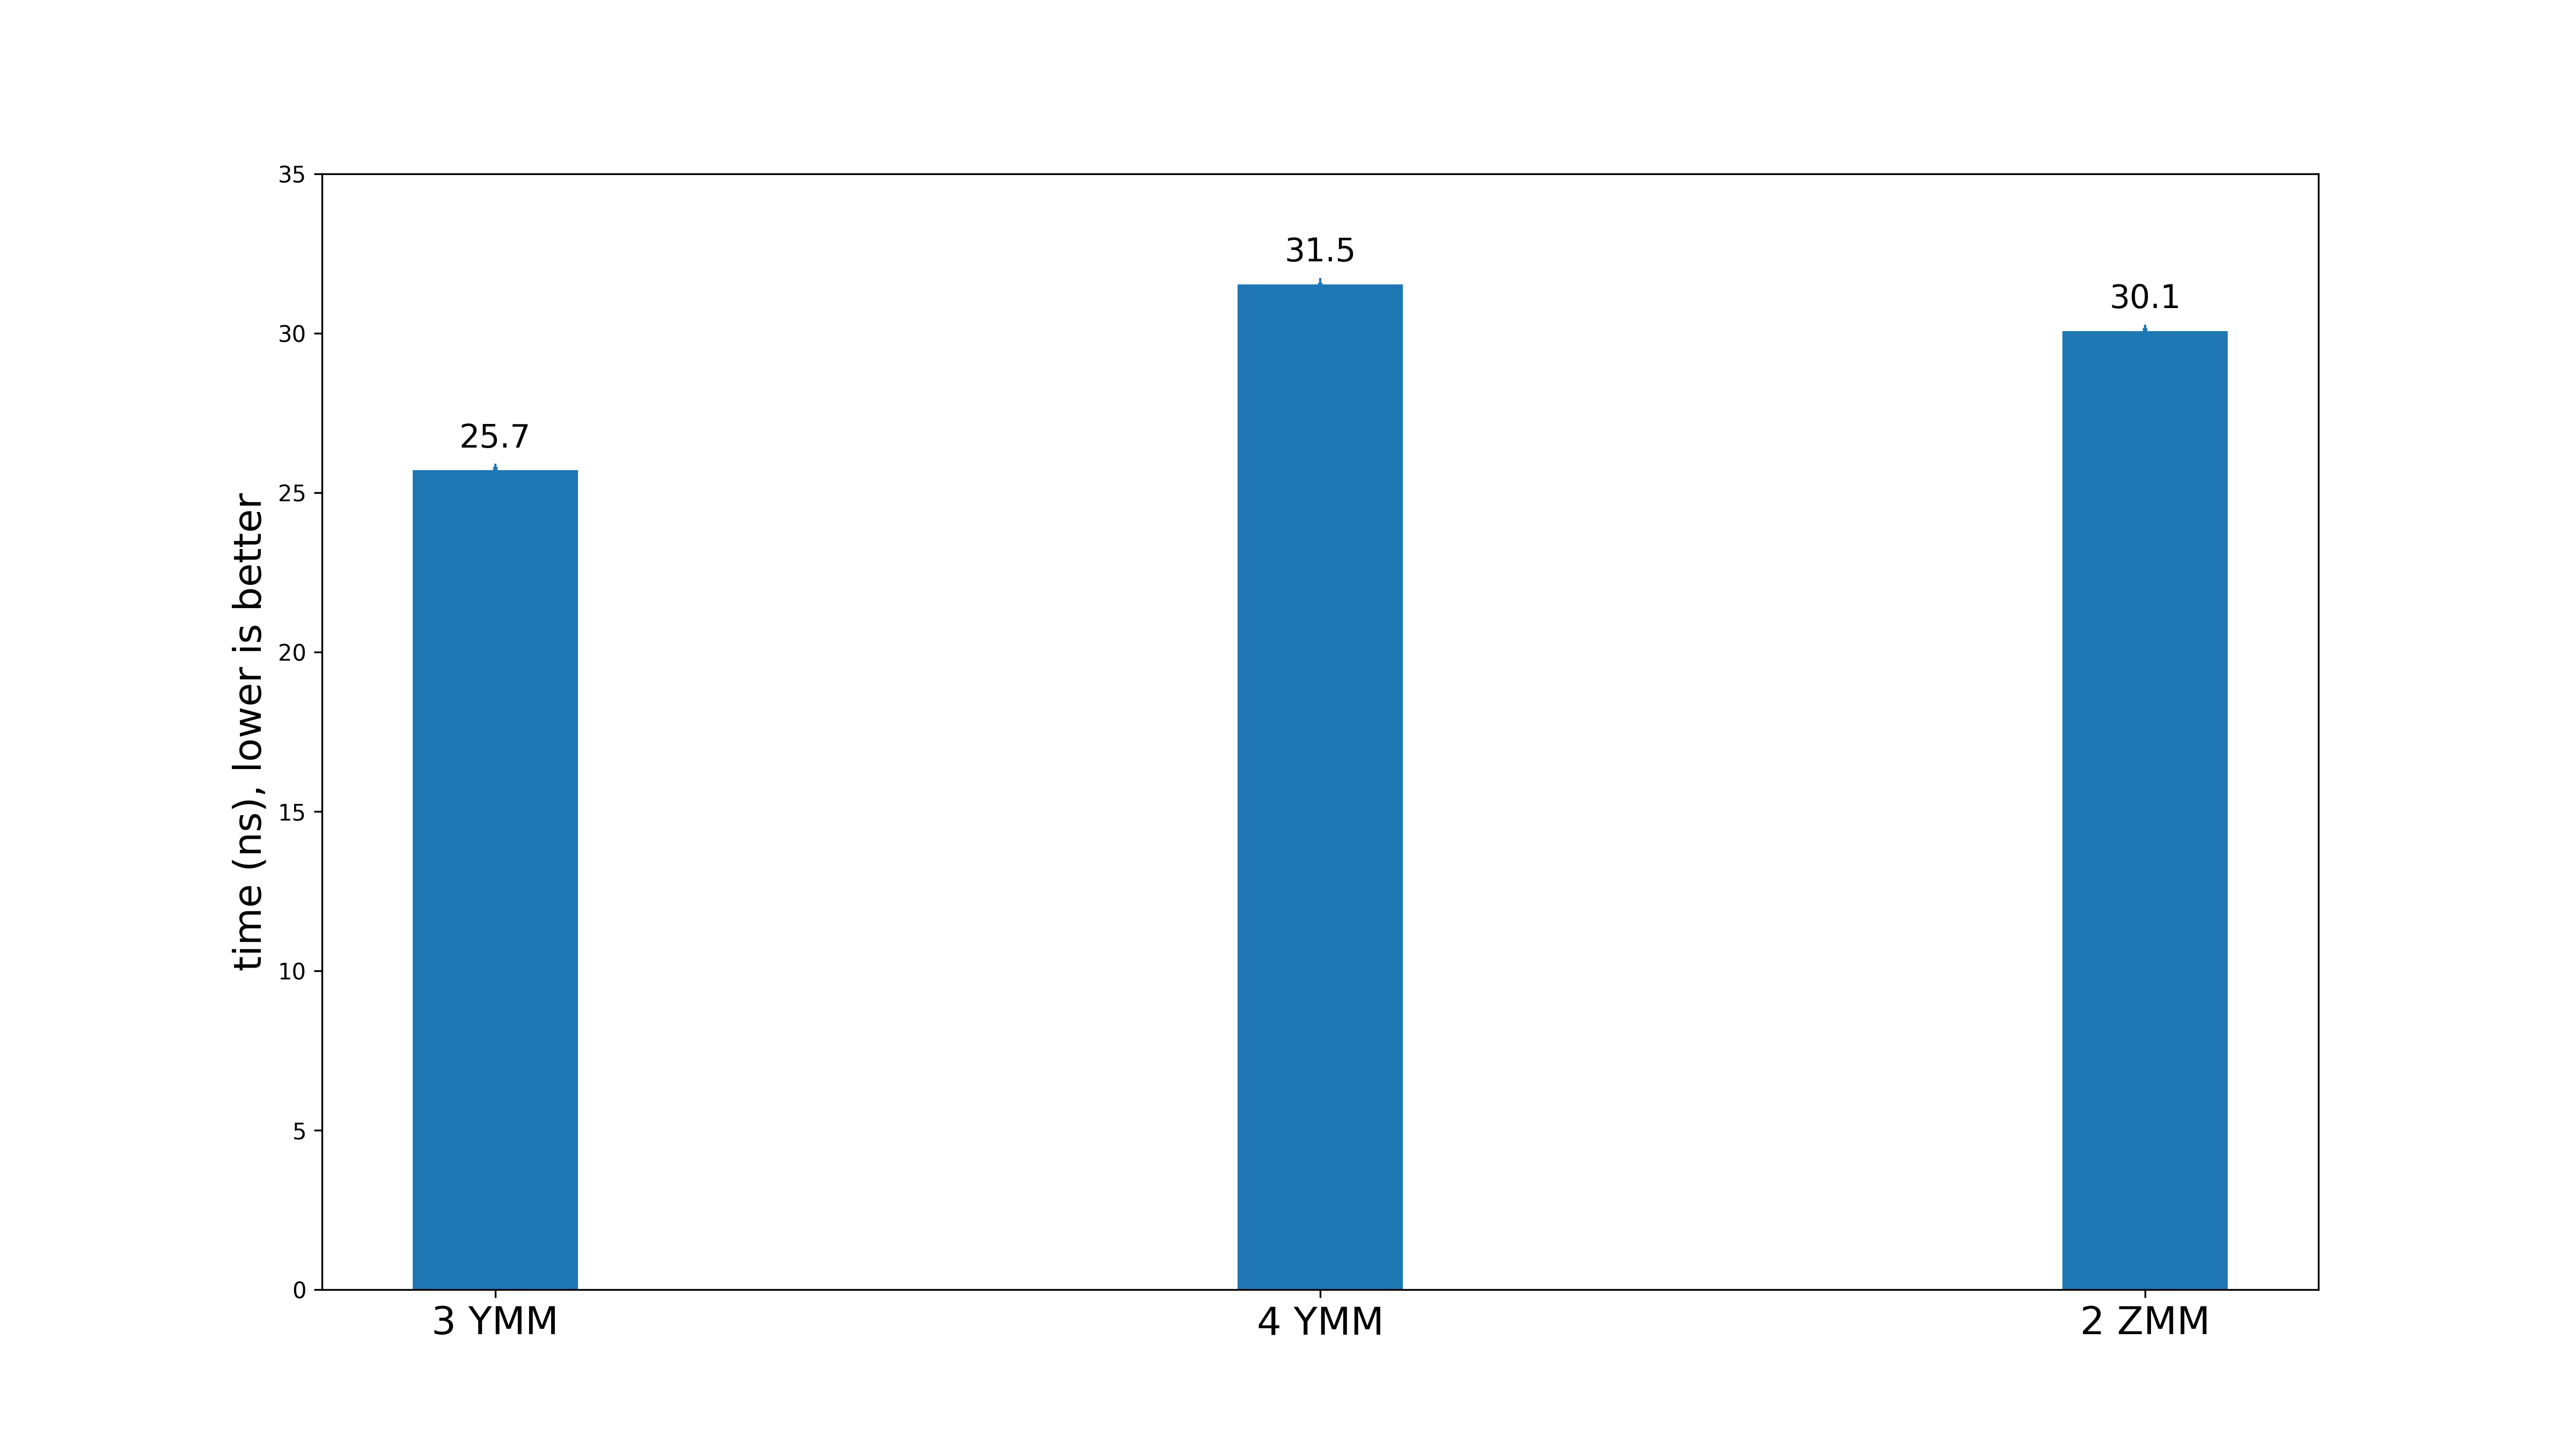
\includegraphics[width=\linewidth]{image/3ymm-4ymm-2zmm.png}
    \end{center}
    \caption{This benchmark of the \pivot{} function measures the difference in
    performance when rows are packed into 3 \ymm{} vectors, 4 \ymm{} vectors or 2 \zmm{}
    vectors. Apart from them 3 \ymm{} setup is the fastest, It is also worth noting
    that the performance of the 4 \ymm{} implementation is consistently 1.4 ns
    slower than its \zmm{} counterpart. This confirms with Zen 4's performance
    in Section \ref{sec:avx512} that equal amount of workload compiled to
    AVX-512 instructions is faster than AVX-2, due to less front-end pressure.  
    }
    \label{fig:3ymm-4ymm-2zmm}
\end{figure}








\section{Evaluation}
\begin{figure}[H]
    \begin{center}
        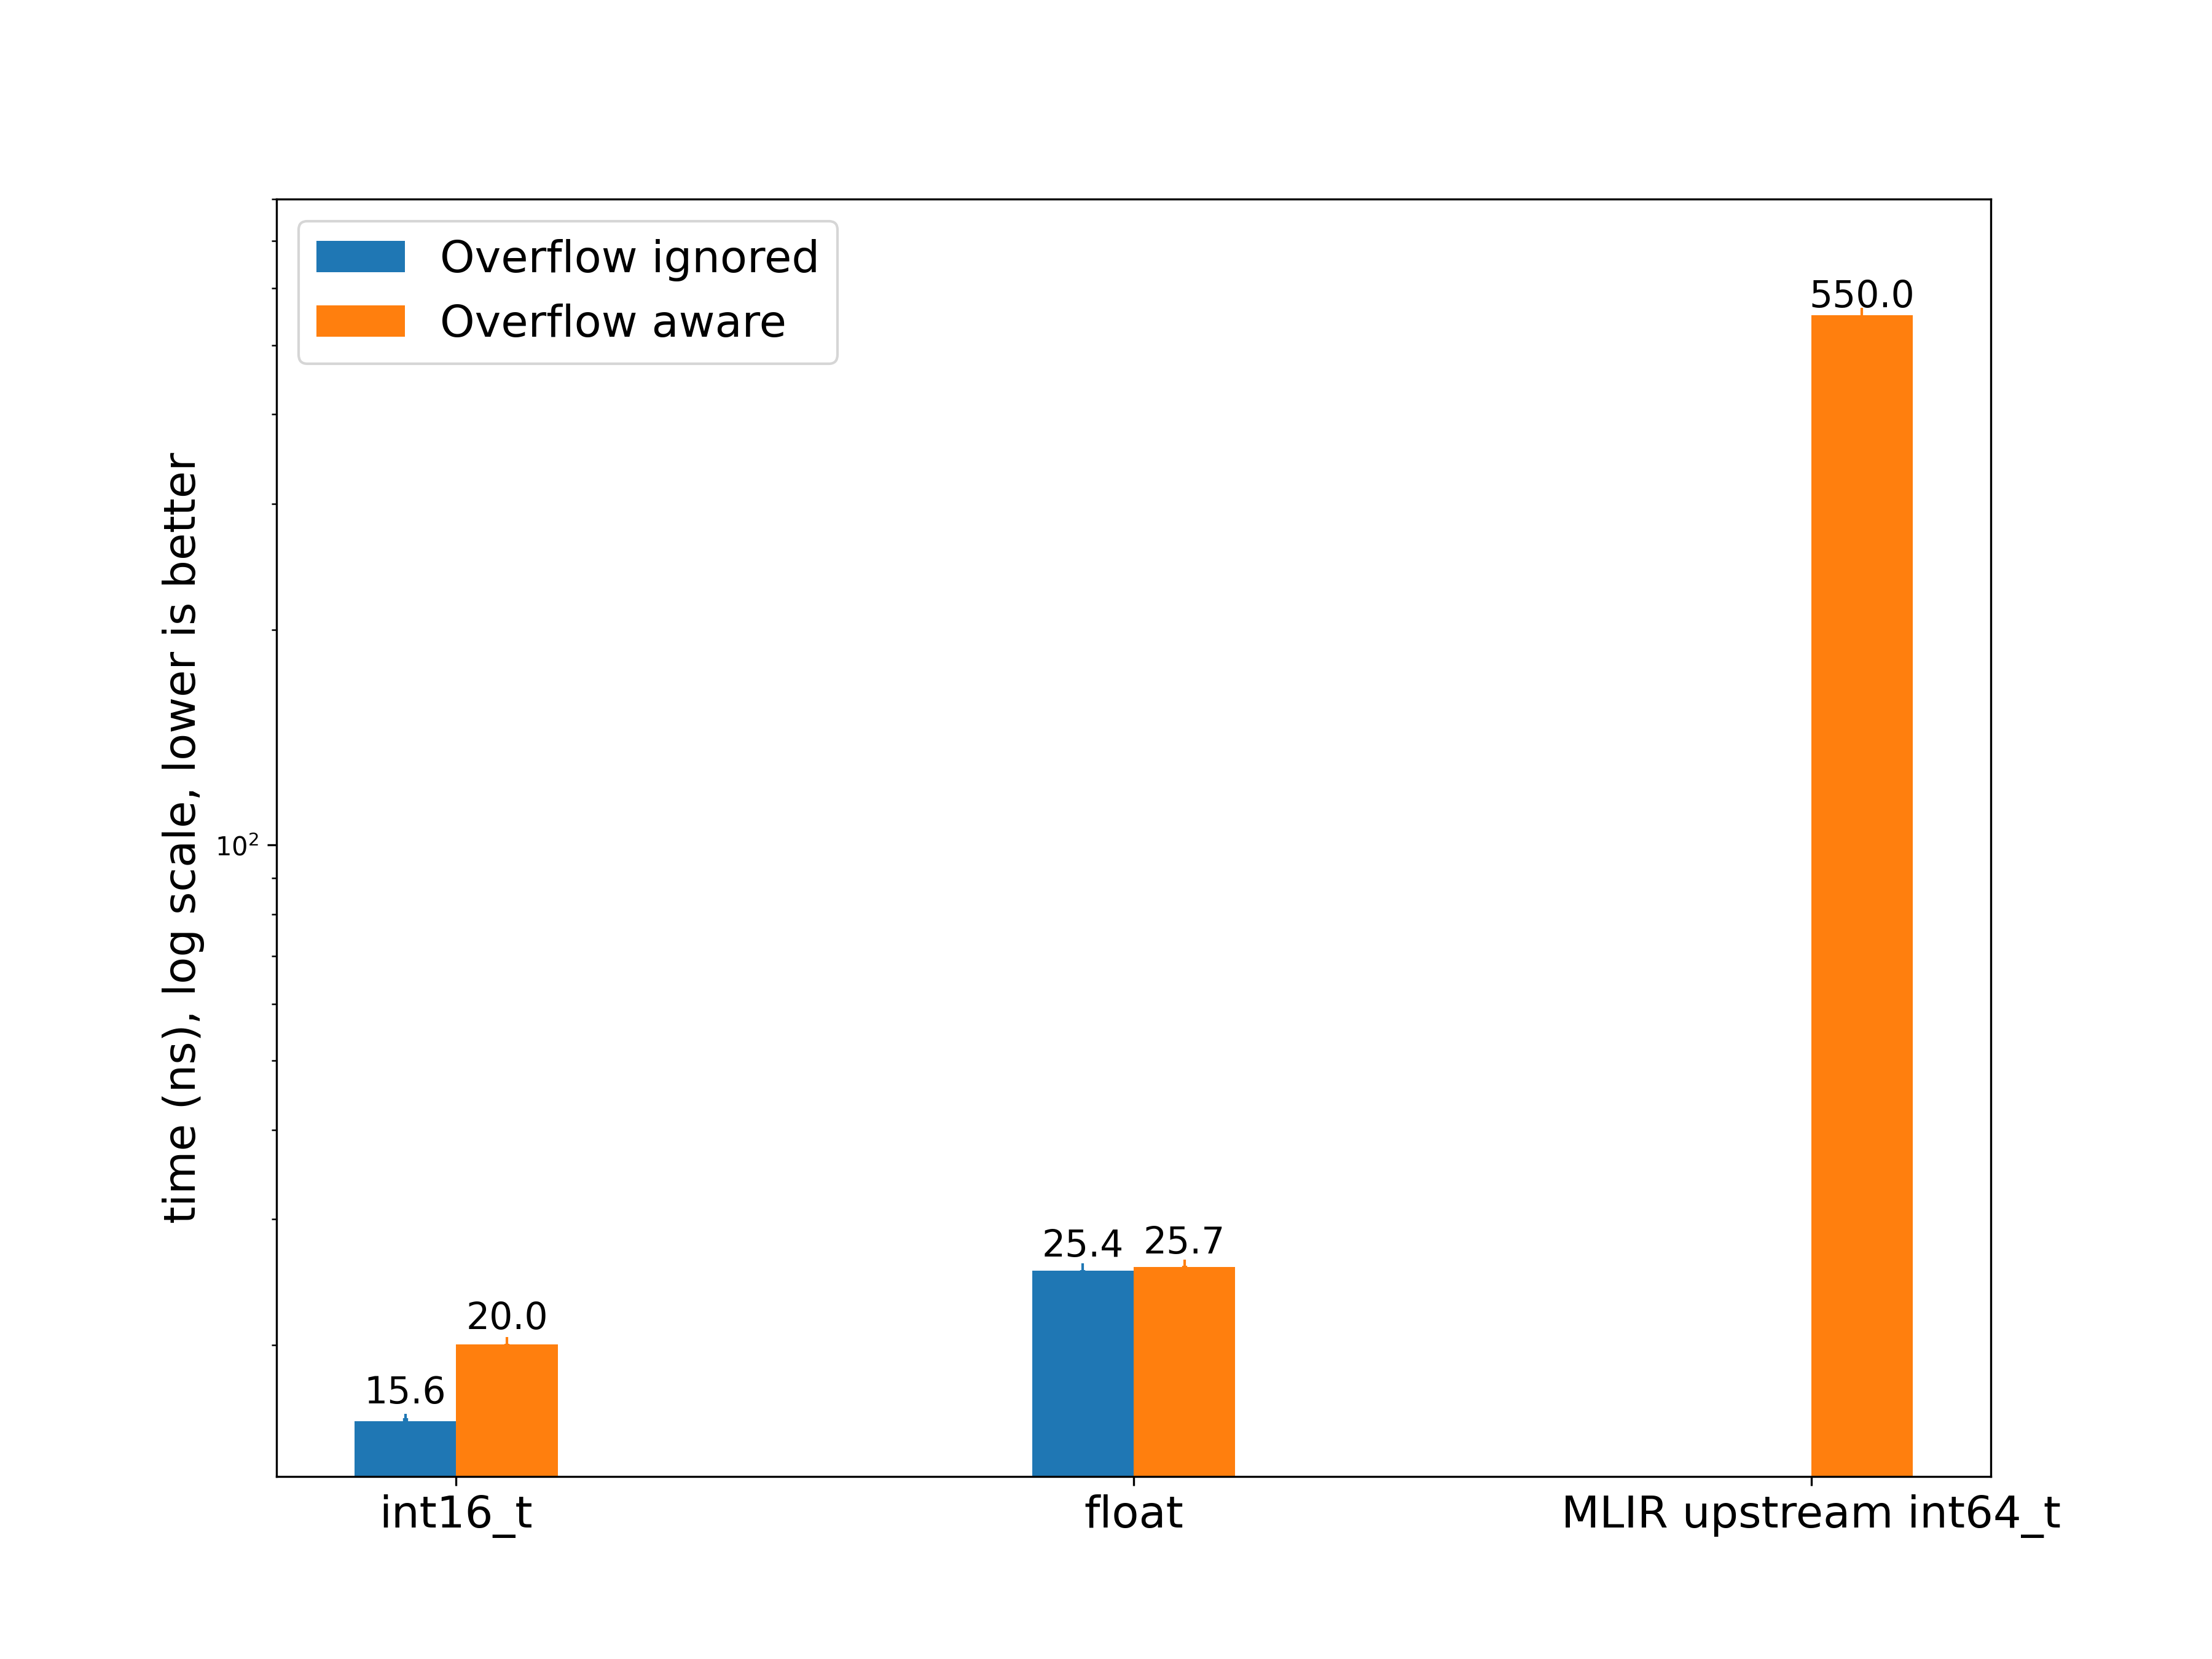
\includegraphics[width=\linewidth]{image/i16-3ymmf32-upstream-overflow.png}
    \end{center}
    \caption{ 114514
    }

    \label{fig:i16-3ymmf32-upstream-overflow}
\end{figure}

\begin{figure}[H]
    \begin{center}
        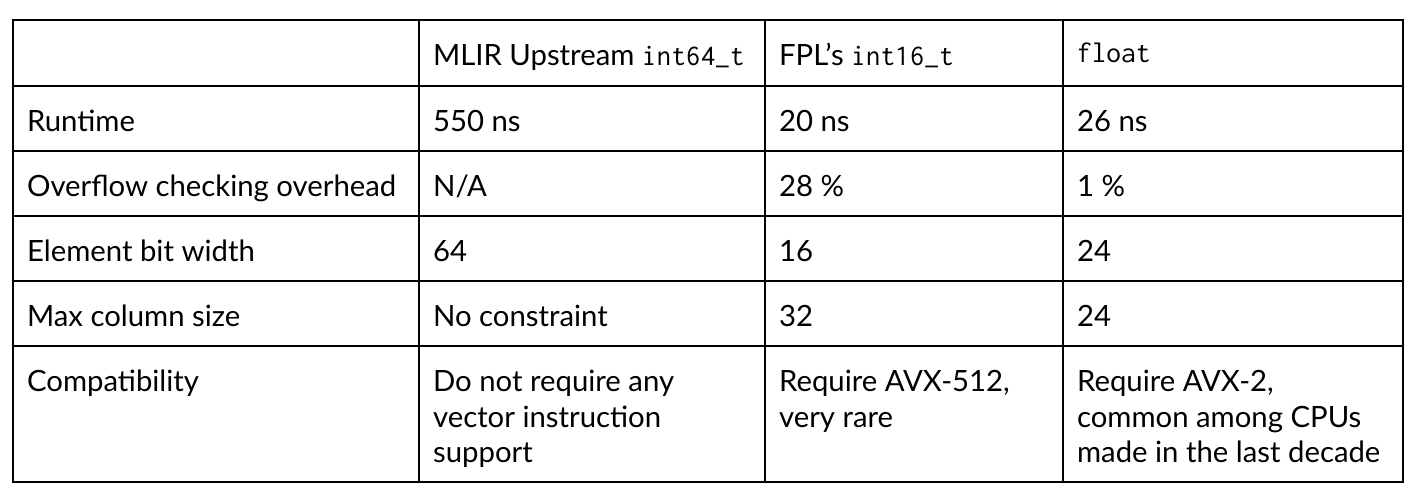
\includegraphics[width=\linewidth]{image/i16-3ymmf32-upstream-table.png}
    \end{center}
    \caption{ 114514
    }
    \label{fig:i16-3ymmf32-upstream-table}
\end{figure}

    % \caption{ A benchmark of the \pivot{} function.
    % All implementations using \zmm{} require padding column size to 32.
    % However, the combination of \dtfloat{} and \ymm{} allows some flexibility
    % in padding size. 
    % In cases where the column size is less than 24, instead of padding to 32, 
    % the column size is padded to 24, and three \ymm{} registers are allocated for each row.
    % This approach has been found to be 15\% faster than its \zmm{} counterpart.
    % }
It is discovered from that:
\begin{enumerate}
    \item The \dtshort{} approach from FPL~\cite{FPL2} costs 20 ns, this is 6 ns
    faster than the \dtfloat{} approach proposed by this report. A possible
    reason is that Zen 4 is more capable of doing arithmetics than memory
    IO~\cite{Zen4Critique}. The algorithm using \dtfloat{} could be IO-bounded. 
    \item The benchmark confirms the expectation in Section
    \ref{sec:ColumnSizeSpecialization}.
    \item For Zen 4, migrating AVX-2 code to AVX-512 indeed
    brings some performance increments. The \pivot{} function using \dtfloat{}
    and 2 \zmm{} for a row is 1.4 ns faster than the one using 4 \ymm{} for a
    row. The benchmark confirms the theoretical benefit of AMD's implementation
    on AVX-512 mentioned in Section \ref{sec:avx512}.

\end{enumerate}

% unfortunately \dtfloat{} does not provide a performance advantage over \dtshort{}.
% Specifically, \dtfloat{} takes 26 ns, while \dtshort{} completes 6 ns ahead.
% Nevertheless, both of them significantly outperform the upstream scalar
% implementation, which renders the 6 ns gap trivial. 
% Additionally, \dtfloat{} offers substantial compatibility advantage
% over \dtshort{} for vast amount of non-AVX-512 platforms. 



\chapter{Conclusion and Future Work}

In conclusion, this report presents a fast implementation of the \pivot{}
function using \dtfloat{} to address performance bottlenecks when MLIR analysis
programs using linear programming of the simplex method. The procedures are: 
\vspace*{-2.2mm}
\begin{compactlist}
    \item Write source code using Clang's vector type extension to guarantee
    vectorization.
    \item Reduce the bit width of each element in the input matrix.
    High-precision data types are unnecessary for \pivot{}.
    \item Perform integer arithmetics with FPU to leverage floating point's
    automatic overflow detection.
\end{compactlist}

I achieved 20 times speedup over the upstream implementation, but unfortunately,
it is about 20\% slower than the FPL's approach. Nevertheless, my method offers
better compatibility. The FPL's approach requires AVX-512, but mine works on old
and vastly more common AVX-2 CPUs.


My techniques of optimizing the \texttt{pivot} function could make further
progress with the 16-bit floating point data type \dthalf{}. It consists of
a 1-bit sign, a 5-bit exponent, and a 10-bit mantissa (Figure
\ref{fig:ieee-f16}). For some AI applications where high precision is not
needed, \dthalf{} provides performance benefits over \dtfloat{} and
\dtdouble{}~\cite{fp16-fast}. It has been supported natively on GPUs since
2016~\cite{pascal-intro-fp16}, and if this data type is integrated into future
AVX extensions, it would potentially further improve the performance of
\pivot{}. The \dthalfi{} data type can be defined using the 10-bit
mantissa, which covers 99\% of the elements in the constraint
matrices~\cite{FPL1}. It is expected to improve the runtime of the \pivot{}
function by 2 times if \dtfloati{} is replaced with \dthalfi{}.

%  overflow-ignored version, and the runtime
% can be reduced to about 50\% comparing to the \pivot{} function implemented
% using \dtfloat{} in this report.

\begin{figure}[H]
    \begin{center}
    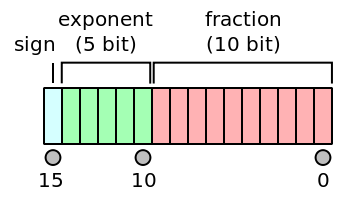
\includegraphics[width=50mm,scale=0.1]{image/ieee-f16.png}
    \end{center}
    \caption{IEEE 754 half precision floating point (16 bits)~\cite{fp16-diagram}.}
    \label{fig:ieee-f16}
\end{figure}


\chapter{Related Work}
\begin{enumerate}
    % \item mlir
    \item ISL
    \item fpl
    \item cache modeling paper
    
    \item \textbf{Fast Modular Exponentiation using Floating Point Arithmetic in
    GPU}~\cite{intfpu-modexp}: Modular exponentiation is critical to RSA
    cryptographic operations. It is the calculation of the remainder $r$ when an
    integer $b$ is raised to the power of $e$, then divided by the modulus $m$:
    $r = b ^ e$ mod $m$. The paper presents an approach of computing modular
    exponentiation using double precision floating points, and achieved 20\% to
    34\% speed up over the best prior implementation.
    
    \item \textbf{Transprecision Training Using \dthalf{} and
    \dtfloat{}}~\cite{fp16-fast}: Performance and memory efficiency of deep
    learning models can be improved by starting with low precision \dthalf{}
    arithmetics, and switch to \dtfloat{} if high precision is required. NVIDIA
    advertises 8 times more \dthalf{} arithmetic throughput when compared
    to \dtfloat{}, and this translates into 2 to 4.5 times speedup 
    for transprecision models.
\end{enumerate}

% \section{Final Reminder}

% The body of your dissertation, before the references and any appendices,
% \emph{must} finish by page~40. The introduction, after preliminary material,
% should have started on page~1.

% You may not change the dissertation format (e.g., reduce the font size, change
% the margins, or reduce the line spacing from the default single spacing). Be
% careful if you copy-paste packages into your document preamble from elsewhere.
% Some \LaTeX{} packages, such as \texttt{fullpage} or \texttt{savetrees}, change
% the margins of your document. Do not include them!

% Over-length or incorrectly-formatted dissertations will not be accepted and you
% would have to modify your dissertation and resubmit. You cannot assume we will
% check your submission before the final deadline and if it requires resubmission
% after the deadline to conform to the page and style requirements you will be
% subject to the usual late penalties based on your final submission time.

\bibliographystyle{plain}
\bibliography{mybibfile}


% You may delete everything from \appendix up to \end{document} if you don't need it.
% \appendix

% \chapter{First appendix}

% \section{First section}

% Any appendices, including any required ethics information, should be included
% after the references.

% Markers do not have to consider appendices. Make sure that your contributions
% are made clear in the main body of the dissertation (within the page limit).

% \chapter{Participants' information sheet}

% If you had human participants, include key information that they were given in
% an appendix, and point to it from the ethics declaration.

% \chapter{Participants' consent form}

% If you had human participants, include information about how consent was
% gathered in an appendix, and point to it from the ethics declaration.
% This information is often a copy of a consent form.


\end{document}
